%\documentclass[10pt,a4paper,english]{article}
\documentclass[12pt, a4paper]{article}
\usepackage[utf8]{inputenc}
\usepackage[T1]{fontenc}
\usepackage[margin=2.5cm,top=2.5cm, bottom=2.0cm]{geometry}
\usepackage[english]{babel}
%\usepackage{lmodern}
\usepackage{newtxtext}
\usepackage{newtxmath}
\usepackage[fleqn]{mathtools}
\usepackage{amssymb}
\usepackage{dcolumn}
\usepackage{siunitx}
\usepackage[official]{eurosym}
\setcounter{secnumdepth}{3}

\usepackage[babel=true]{microtype}
\usepackage[hang]{footmisc}
\usepackage[usenames,dvipsnames,svgnames,table]{xcolor}

\usepackage[format=hang, justification=RaggedRight]{caption}
\usepackage[section]{placeins}
\usepackage{float}
\usepackage{booktabs}
\usepackage{comment}
\usepackage{graphicx}
\usepackage{epstopdf}
\usepackage[layout=margin,author=,status=draft]{fixme}
 \usepackage[final]{changes} %Manually track changes
 \definechangesauthor{SKB}
\usepackage{longtable}
\usepackage{paralist}
\usepackage{rotating}
\usepackage{subfigure}
\usepackage[natbibapa]{apacite}
%\usepackage[authoryear]{natbib}
\usepackage{csquotes}
%modifying the thanks commands
\usepackage{titling}
\usepackage[colorlinks=true, urlcolor=blue, citecolor=black, linkcolor=black]{hyperref}
\usepackage[noabbrev,capitalise]{cleveref}

\DeclareUnicodeCharacter{2010}{-}% support older LaTeX versions
\thanksfootextra{}{\hfill}
\setlength{\thanksmargin}{1em}
\setlength{\thanksmarkwidth}{0.75em}

\fxsetup{theme=color}
%Custom commands
\newcommand{\eur}{\EUR}
\newcommand{\std}[1]{\emph{(#1)}}
\newcommand{\V}{\checkmark}
\def\fns{\footnotesize}
\renewcommand*{\vec}[1]{\boldsymbol{#1}}

\def\tenpc{$^{\ast}$}
\def\fivepc{$^{\ast\ast}$}
\def\onepc{$^{\ast\ast\ast}$}
\newcommand{\legend}{\normalsize{Significance levels:\hspace{1em} \tenpc : 10\% \hspace{1em} \fivepc : 5\% \hspace{1em} \onepc : 1\% \normalsize}}
\def\sep{0.5em}
\def\legendTwo{\multicolumn{3}{l}{\footnotesize{Significance levels
			:\hspace{1em} $\dag$ : 10\% \hspace{1em}
			$\ast$ : 5\% \hspace{1em} $\ast\ast$ : 1\% \normalsize}}}
\def\sym#1{\ifmmode^{#1}\else\(^{#1}\)\fi} % needed for the tables produced by the esttab command in Stata, to avoid redundancy put here instead of in appendix.tex, where it is needed		
%SKB: Added for documenting the tables and figures
\newcommand{\modelTwo}{age, age\textsuperscript{2}, education, marriage, number of children, inter-ethnic household}
\newcommand{\modelThree}{\modelTwo, industry, occupation, ownership type of company, number of workers in company, working in the public sector, experience in company}
\newcommand{\industry}{Industry categories (according to NACE Rev.2): A Agriculture, Forestry and Fishing; B Mining and Quarrying; C Manufacturing; D Electricity, Gas, Steam and Air Conditioning Supply; E Water Supply;  Sewerage, Waste Management and Remediation Activities; F Construction; G Wholesale and Retail Trade;  Repair of Motor Vehicles and Motorcycles; H Transportation and Storage; I Accommodation and Food Service Activities; J Information and Communication; K Financial and Insurance Activities; L Real Estate Activities; M Professional, Scientific and Technical Activities; N Administrative and Support Service Activities; O Public Administration and Defence;  Compulsory Social Security; P Education; Q Human Health and Social Work Activities; R Arts, Entertainment and Recreation; S Other Service Activities; T Activities of Households as Employers;  Undifferentiate Goods and Services Producing Activities of Households for Own Use; U Activities of Extraterritorial Organisations and Bodies}
\newcommand{\occupation}{Occupation categories according to ISCO-08: 1 Managers; 2 Professional; 3 Technicians and associate professionals; 4 Clerical support workers; 5 Service and sales workers; 6 Skilled agricultural, forestry and fishery workers; 7 Craft and related trades workers; 8 Plant and machine operators, and assemblers; 9 Elementary occupations; 10 Armed forces occupations}
\newcommand{\modelThreeAdd}{industry, occupation, ownership type of company, number of workers in company, working in the public sector, experience in company}	
\newcommand{\restrictions}{The sample period is from year 2000 to year 2012. Sample is limited to persons 25-55 year old.}
\newcommand{\agerestrictions}{25-55 year olds only.}
% Modified section numbering: removed dot at the end as this jumps
% into the cross-references.
\renewcommand{\thesection}{\arabic{section}}
\renewcommand{\thesubsection}{\thesection.\arabic{subsection}}

\title{Language Skills in an Ethnically Segmented Labour market:
 Estonia 1989 -- 2012}
%\author{Sven-Kristjan Bormann \and Svetlana Ridala\thanks{Acknowledgements: 
%This research was supported by European Social Fund's Doctoral Studies
%and Internationalisation Program DoRa through Archimedes Foundation, and the Estonian Science Foundation grant 8627.} 
%\and Ott Toomet
%}
\date{}
\begin{document}

%\maketitle
%\begin{center}
%	\textbf{{\large Language Skills in an Ethnically Segmented Labour market:
%				Estonia 1989 -- 2012}} \\
%	{\large Sven-Kristjan Bormann} \\
%	\emph{School of Economics and Business Administration, University of Tartu, Narva mnt. 4, 51007 Tartu, Estonia\\ Tel.: +372 5844 3873\\ Email: \href{mailto:bormann@ut.ee}{bormann@ut.ee}}	\\
%
%	{\large Svetlana Ridala} \\
%	\emph{School of Business and Governance, Tallinn University of Technology, Akadeemia tee 3, 12618 Tallinn, Estonia\\ Email: \href{
%			mailto:svetlana.ridala@gmail.com}{
%			svetlana.ridala@gmail.com}} \\
%		{\large Ott Toomet}\\
%		\emph{Information School, University of Washington, USA; Email: \href{mailto:otoomet@uw.edu}{otoomet@uw.edu}}
%%	\emph{(Received XX XXXX 20XX; accepted XX XXXX 20XX)}\\
%	\textbf{Corresponding author:} Sven-Kristjan Bormann Email: \href{mailto:bormann@ut.ee}{bormann@ut.ee}
%\end{center}
%\paragraph{Short biographical note:} \hspace{0pt} \\
%Sven-Kristjan Bormann born 28.11.1985, graduated in 2011 from Kiel University, Germany in Economics with specialisation in Quantitative Economics and Computer Science. Since September 2012 PhD-student in Economics at Tartu University, Estonia. \\
%Svetlana Ridala born 28.03.1976, graduated in 2003 from Tallinn Pedagogical University, Estonia master's (scien) degree in mathematics. Since 2009 PhD-student in Economics at Tallinn School of Economics and Business Administration, Estonia.
%\\
%Ott-Siim Toomet born 18.03.1970, graduated in 2004 from Aarhus University, Denmark PhD in Economics. Since 2015 Visiting scholar, Information School, University of Washington.
%
%\paragraph{Research funding}
%This research was supported by European Social Fund's Doctoral Studies
%and Internationalisation Program DoRa through Archimedes Foundation, and the Estonian Science Foundation grant 8627.
%\newpage
%\noindent
{\centering \textbf{Language Skills in an Ethnically Segmented Labour Market: Estonia 1989 -- 2012}}
\begin{abstract}
 \noindent
 \textbf{Purpose --} We analyse the relationship between skills in the
 Estonian, Russian and English language, and labour market
 outcomes in Estonia, a linguistically divided country.
 \\
 \textbf{Design/methodology/approach --} We use the Estonian Labour
 Force Surveys 1992--2012. We rely on multivariate linear regression
 models to document the relationship between language skills and
 labour market outcomes.
 \\
 \textbf{Findings --} Estonian language knowledge (for ethnic Russians)
 are important determinants of unemployment. Wage, in contrary, is
 closely related to English skills. Ethnic Russian men do not earn
 any premium from speaking Estonian, while women, fluent in Estonian
 earn approximately 10\% more. For ethnic Estonians, Russian fluency
 is associated with a similar income gain.
 \\
 \textbf{Research limitations/implications -- } Due to the
 observational nature of the data, the effects reported in our study
 are not causal effects. As a second limitation, the self-reported
 language skills data may be imprecise and hence the effects we
 report may be too small.
 \\
 \textbf{Practical implications --} Our results stress the role of
 workplace segregation, both along gender and ethnic lines, in
 determining the individual labour market experience. 
 \\
 \textbf{Originality/value --} We provide a comprehensive overview of
 the effects of language skills in a rapidly developing labour
 market in a linguistically divided economy. We analyse several
 languages with different legal status and document long-term
 trends in the effects.
 \\
\end{abstract}
\textbf{Keywords:} language skills, ethnicity, wage gap, unemployment, Estonia \\
\textbf{JEL classification:} J15, J31, J71


\section{Introduction}
\label{sec:introduction}
Numerous studies document that language skills are related to better
labour market outcomes.
Speaking different languages may make workers genuinely more
productive, either by facilitating communication at the workplace
or by making it possible to perform
tasks that require language knowledge.
Enhanced productivity, in turn, should be reflected both in better wage
and in improved employment prospects.

The bulk of the existing literature analyses the effect of knowledge
of the local majority language for immigrants. It is well known that
language skills are associated with an income premium
between 5 and 35 percent
\citep{Chiswick1995,bleakley+chin2004,shields+price2002,leslie+lindley2001,chiswick+miller2002,Chiswick2010,Chiswick2015, Dustmann2003}. For
instance, \citet{chiswick2008} argues that ``proficient'' speakers
typically earn about 15\% more than ``not proficient'' speakers.
The effect works largely through improving educational attainment
\citep{bleakley+chin2004,rooth+saarela2007native}. Language skills are
also complementary to other types of human capital
\citep{chiswick+miller2007}.
Immigrants who are fluent in the local language also suffer
substantially less from unemployment \citep{shields+price2002, Dustmann2003}.



However, in the case of less-than-perfect ethnic integration, the ``local''
language in ethnic enclaves may be the minority language instead, in
this way limiting the usefulness of the majority language skills
\citep{chiswick+miller2002,hwang+2010} in particular in context of ethnic segregation and
limited access to upper-end jobs \citep{Toomet2011}. However, the
existing evidence suggests that the majority language is
an important production factor in the ethnic enclaves as well
\citep{zhou+logan1989, clark+drinkwater2000}.


There is also an increasing body of literature focusing on other languages than the local main business language. These studies generally find
that English is a significant predictor of better income
\citep{Lang2009, Casale2011, Toomet2011, Williams2011, azam+2013EDandCC, isphording2013, fabo+2017E}.
The role of other languages, in particular in a multi-lingual economy, is
less clear. For instance,
\cite{Drinkwater1997} finds
a positive effect for Welsh speaking workers in
Wales and \cite{Armstrong2015} shows that bilingual native French-speakers enjoy
a significant premium both inside and outside of Quebec.
\citet{FrancoisGrin1998}, in contrast,
shows that Italian language skills in Swiss non-Italian speaking
regions are associated with a lower wage. It remains unclear if
this is a true effect or just an omitted variable bias.

Few previous studies have provided a comprehensive analysis of a labour
market from the viewpoint of language skills.
\citet{Chiswick1995, chiswick+miller2002, chiswick+miller2007,
 Bellante1998, Chiswick2010} analyse the effects of dominant language
fluency for earnings among immigrants in the United States, 
\citet{Chiswick1995} also do this for Canada, Australia and Israel.
\citet{leslie+lindley2001} analyse both employment and income but
focus on a single year and English language only.
\citet{YaoandOurs2015} only analyse the role of Dutch language
on labour market performance in the Netherlands. 

The literature on Central Eastern Europe (CEE) and former Soviet Union
countries is rather limited. We know that the different development
trajectories have led to disparities both favouring the Russian-speaking
minority in Ukraine \citep{Constant2011} and hindering them in Estonia
\citep{Leping2008}. \citet{Kahanec2009} show that non-citizens suffer
less favourable outcomes, in particular, ethnic Russians in Estonia and
Latvia. 
\cite{Alan2015} show that Russian language proficiency is valuable in
the former USSR republic in the Caucasus (Armenia, Azerbaijan and
Georgia) by increasing employment likelihood between six and nine
percentage points. \citet{Toomet2011}, however, fails to find any
income premium from the majority language fluency in Estonia and
Latvia. This outcome is corroborated by \citet{Lindemann2013} who shows that Estonian fluency
is associated with faster job finding rate while it does not
explain the lower occupational prestige of Russian speakers. 
A number of these studies have to overcome severe data limitations,
such as lack of fine-grained information on ethnic background in
EU-wide surveys \citep{Kahanec2010}.

In this paper, we analyse the relationship between both
majority and minority language skills, and English for both
wage and unemployment. We analyse Estonia, a former Soviet republic
and now a rapidly growing and
transforming Easter European country. It is characterized by a stark linguistic division
where the Russian-speaking community forms almost 30\% of
the population. We use the Estonian Labour Force Survey, one of the
higher-quality long-term datasets, well suitable for our
purpose. We provide long--term trends from the last years
of the planned economy in 1989 till the post-recession time in 2012.

We find that the Estonian language, the ethnic majority and official
language of the country, is associated with a very
small albeit slowly increasing wage premium over
the years. Interestingly, this is true only for women, Russian men enjoy
virtually no premium from the majority language skills.
Russian skills, on the other hand, are clearly related to
higher wage but the relationship is slowly fading. English fluency was
associated with a very large wage premium during the early years of
economic transition, later its importance
declined but remained sizeable. 
In contrast, the sole language that plays a role in determining
unemployment probability is Estonian. Its fluency is associated with 
approximately 5 percentage points lower probability of being unemployed.
These results suggest that the Estonian labour market is 
segmented both along gender and the along ethnic background, with men
more likely occupied in less communication-intense jobs.


The paper continues as follows: The next section provides a brief
background of Estonian society and the labour market. In the following
section, we discuss the data and provide some descriptive
statistics. In \cref{sec:method} we describe the econometric
approach, sections \ref{sec:results} and \ref{sec:extensions} present
the results for unemployment probability and wages. The two last
sections, \ref{sec:segregation-analysis} and \ref{sec:discussion}, are
devoted to an additional analysis of labour market segregation, and
concluding discussion.


\section{Background: Ethnic Groups and Languages in Estonia}
\label{sec:hist_background}

This section briefly reviews the institutional and economic background
in Estonia, a country of 1.3M inhabitants,
focusing on the role of ethnic groups and languages.
See \citet{Leping2008} and
\citet{lindemann+saar2011Russian2ndGeneration} for more detailed information.

Before the Second World War, the country was ethnically rather
homogeneous with 90 percent of the population being ethnic Estonians. After the War,
the Russian-speaking population grew rapidly through migration and
reached 40\% by 1989. The migrants largely settled in Ida-Virumaa, a
mineral-rich industrial area in North-East of the country, and in the
metropolitan area near the capital city Tallinn. The
Russian-speakers are still very unevenly distributed.

Such an influx of mainly
Russian-speaking population
led to two \emph{de facto} official languages
by 1970s.
The society was largely divided across language, and the division was
also reflected at workplace \citep{leppik+vihalemm2015JofBaltStud}.
Certain sectors in the economy, such as the armed forces, railways and the
merchant fleet
were dominated by
Russian-speaking workers while more local industries,
such as agriculture and
public administration,
were dominated by ethnic Estonians.
Both communities followed the media in their own respective language, the
universities taught many subjects in both Russian and Estonian,
and service sector was largely bilingual. However, the bilingualism
was mainly one-sided as the bulk of Estonians spoke Russian, but not
the other way around. A particular institution in parts of the Soviet
Union was a segregated school system, where Russian schools existed along the
schools teaching in the local language. Hence, a common education
system, one of the central integration mechanisms in the developed world,
was (and still largely is) missing in Estonia.
The widening use of Russian also
caused increasing concerns about the future of the Estonian
language, in turn leading to an unwillingness to use Russian by
the ethnic Estonians. This further strengthened the language-based segregation.

When the central Soviet authority weakened during the late 1980s, the
Estonian-speaking community was quick to organize and established a
nation-state in 1991 where
Estonian was granted status as the sole official language. The
above-mentioned ``one-sided bilingualism'' started turning
around. The universities quickly moved to Estonian-only curriculum,
the Estonian language became a compulsory subject in Russian schools
while teaching Russian in Estonian-language schools declined.
These trends have continued until today, according to
\citet{HTM2015}, one quarter of the students from non-Estonian-speaking families studied in Estonian schools.
As a result, the younger generation of ethnic Estonians is
increasingly less fluent in Russian while the ethnic Russians are
steadily getting better in Estonian.

The Estonian economy, a part of the Soviet economy up to 1991, successfully
re-oriented to the Western markets and has been growing rapidly since
the mid-1990s. 
\Cref{fig:gdp_growth} shows that it grew averaged at approximately 7\%
annually
before the financial crisis in 2008, afterwards the figure has been around 3\%.
As a by-product of the re-adjustment, English skills become extremely
valuable while the supply was still rather limited during the early
years of the transition.

\begin{figure}[h]
 \centering           
 \caption{Annual GDP growth in Estonia}\label{fig:gdp_growth}
 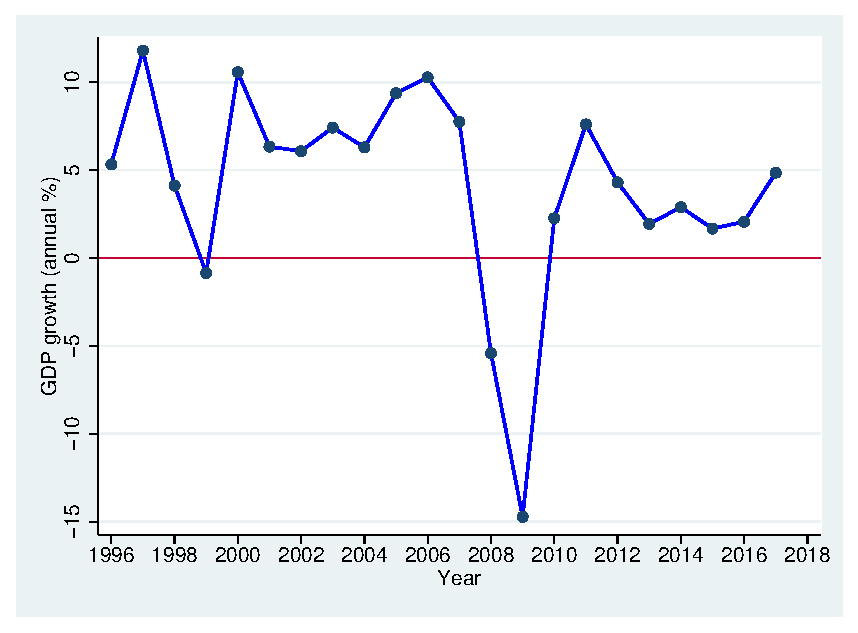
\includegraphics[width=0.6\linewidth]{Figure1.eps}
 \caption*{Source: World Bank - World Development Indicators}
\end{figure}

The economic and political reforms led to substantial
disparities in income and education opportunities
in the early 1990s \citep{Leping2008,
	lindemann+saar2011Russian2ndGeneration}. Inter-ethnic contacts
are largely limited to superficial encounters at work and in public
space, the number of close private ties remain limited
\citep{korts2009JofBaltStud}. The
separate worlds are also reflected in media which may present quite
different and occasionally antagonistic viewpoints depending on the
language \citep{Korts2002}.


\section{Data}
\label{subsec:ss_var}

\subsection{Variables and Sample Selection}
\label{sec:variables}

Our main analysis relies on the Estonian Labour Force Survey (ELFS),
first conducted in 1995 by the Estonian Statistical Office. We limit
ourselves with years 2000--2012 in the main analysis, motivated by a
methodology break: Until 1999 the survey was conducted as an annual
cross-section and later as a quarterly rotating panel. The survey
contains data on approximately 4000 distinct individuals annually,
however, due to its rotating nature, we have roughly 16,000 annual
observations for each year since 2000. For the long-term analysis, we
also use the earlier waves. These waves also include a retrospective
section that contains income up to several years back.

We limit ourselves to men and women in the main working age, between 25 and
55 years old. Further, we only analyse
individuals who are either working or actively looking for a job.
The dataset allows us to control for standard personal
characteristics and human capital variables, such as age, education
and family status. We discuss the most important variables below.

In all waves of the survey, respondents are asked about their
``ethnic nationality''. Typically, individuals have a single ethnic
identity. The answers are coded as ``Estonian'' or
``non--Estonian''. As most of those who do not consider themselves
Estonian use Russian as their primary language, we refer to this group
as ``Russians''.                                  
              
The labour market outcomes we analyse are income, the ``last salary on the main job'' and
labour force status (working, unemployed or inactive). 
                                  
The survey includes self-reported language skills on languages used at
home and all other languages they understand. The respondents are
given some guidance in assessing their skills, they can report either
no knowledge, understanding only, speaking but not writing, writing, or using the
language at home. We consolidate this information into a dummy variable, equal
to one if one speaks or writes, or uses that language at
home, and zero otherwise. Hence, we disregard passive understanding
only.

For further evidence on ethnic and gender segregation at the workplace, we use data
from 2008 Integration Monitor Survey. The survey was conducted by
SaarPoll and focuses on
ethnic relations in Estonia. The sample size is 1500,
500 of the respondents consider themselves not ethnic Estonians. We analyse
two questions: ``which is the language of communication at your
workplace?'' and ``which languages do you need at work''. The first
question addresses the ethnic segregation while the second focuses on
the need for communication.


\subsection{Descriptive Statistics}
\label{sec:descriptive}

The average wages, language skills and other explanatory variables together with the relative frequencies for the period 2000--2012 are presented in \cref{tab:descriptive}. We report the data separately for ethnic nationalities (Estonians and Russians) and language
skills (Estonian, Russian and English).

The table indicates that there are substantial disparities between
Estonians and Russians in wage and unemployment. For instance, the
average monthly salary\footnote{When interpreting these figures,
 one should keep in mind that during this period, 2000-2012, the average monthly salary grow by 180\%,
 from \EUR{314} to \EUR{887} while the language knowledge changed rapidly as
well. However, the ethnic composition of the workforce remained roughly constant.} of Estonian
males who are not fluent in English is \EUR{532} while for Russians it
is only \EUR{452}. However, we also see that Russians who speak
English earn approximately 40\% more than those who do not (\EUR{452}
versus \EUR{326} monthly for men and \EUR{307} versus \EUR{221} for
women). Estonian skills are associated with lower income premium, 15\%
for men (\EUR{378} versus \EUR{329} monthly) and 30\% for women
(\EUR{260} versus \EUR{203}). Analogously, English language skills are more closely
associated with income for Estonians compared to Russian language skills. In
contrast, unemployment shows a different picture. For ethnic Russians,
it is Estonian language fluency that is more closely associated with
low unemployment, those fluent in Estonian have 11.2 percent
unemployment rate while for those not fluent it is 17.3 percent. The
corresponding numbers for English are 11.2 and 15.1. For Estonians,
English is more closely associated with unemployment than Russian:
Estonians fluent in English have on average 5.0 percent unemployment
while those who are not fluent have 8.8 percent. The difference
related to Russian fluency is only 1.6 percentage points. However,
these correlations are not easy to interpret as besides of the strong
time trends, English skills are
also related to education, metropolitan residence, and general
ability.

% Table generated by Excel2LaTeX from sheet 'subgroups_by_ethnic_language'
\begin{sidewaystable}[htbp]
	\centering
	\caption{Averages and relative frequencies of selected explanatory
		variables 2000 -- 2012}
	\begin{tabular}{l|rrrr|rrrr}
		\toprule
		& \multicolumn{4}{c|}{Estonians}  &  \multicolumn{4}{c}{Russians}  \\ \midrule
		Variable          & RUS 0 & RUS 1 & ENG 0 & ENG 1 & EST 0 & EST 1 & ENG 0 & ENG 1 \\ \midrule
		Wage, men (EUR)       & 543.86 & 537.22 & 438.53 & 738.63 & 401.59 & 489.96 & 388.91 & 660.39 \\
		Wage, women (EUR)      & 345.51 & 376.98 & 301.13 & 488.83 & 238.25 & 338.62 & 266.87 & 435.60 \\
		Unemployment (\%)      & 8.74  & 7.13  & 8.83  & 4.99  & 17.30 & 11.18 & 15.06 & 11.23 \\
		EST 1 (\%)         & 99.97 & 99.58 & 99.50 & 99.95 & 0.00  & 100.00 & 40.84 & 80.97 \\
		RUS 1 (\%)         & 0.00  & 100.00 & 77.35 & 82.86 & 99.90 & 99.04 & 99.65 & 98.77 \\
		ENG 1 (\%)         & 29.47 & 37.16 & 0.00  & 100.00 & 6.70  & 30.69 & 0.00  & 100.00 \\
		College Degree (\%)     & 15.61 & 23.44 & 10.77 & 41.38 & 12.66 & 28.64 & 13.93 & 49.16 \\
		Married (\%)        & 40.09 & 55.71 & 54.11 & 49.53 & 63.54 & 60.78 & 63.38 & 56.99 \\
		Inter-ethnic household (\%) & 1.34  & 5.20  & 4.79  & 3.70  & 5.07  & 19.46 & 11.97 & 12.17 \\
		Age             & 37.05 & 41.83 & 42.39 & 38.05 & 42.14 & 40.54 & 42.15 & 37.83 \\
		Kids (number)        & 1.08  & 1.00  & 1.00  & 1.00  & 0.71  & 0.76  & 0.75  & 0.68  \\
		\textbf{Residence County } &    &    &    &    &    &    &    &    \\
		Metropolitan (\%)      & 17.74 & 22.58 & 14.03 & 35.25 & 35.43 & 56.37 & 38.82 & 75.50 \\
		North-East (\%)       & 0.64  & 3.14  & 3.46  & 1.10  & 53.84 & 15.85 & 40.90 & 11.54 \\
		\textbf{Workplace}     &    &    &    &    &    &    &    &    \\
		Tenure (years)       & 6.17  & 7.33  & 7.45  & 6.40  & 8.19  & 7.23  & 8.08  & 5.99  \\
		Public sector (\%)     & 20.03 & 24.81 & 21.79 & 27.55 & 11.62 & 21.67 & 16.28 & 18.14 \\
		Primary sector (\%)     & 14.10 & 9.80  & 13.00 & 6.43  & 9.91  & 7.46  & 8.82  & 8.11  \\
		Secondary sector (\%)    & 31.02 & 27.20 & 32.63 & 19.41 & 47.21 & 29.72 & 41.54 & 24.07 \\
		Tertiary sector (\%)    & 26.17 & 30.12 & 26.52 & 34.46 & 27.17 & 33.96 & 28.37 & 40.96 \\
		\# Observations       & 14,943 & 57,270 & 46,525 & 25,688 & 13,805 & 12,830 & 21,773 & 4,862 \\ \bottomrule
	\end{tabular}%
	\label{tab:descriptive}%
                             
                           
	\caption*{\small
				Workplace--related variables are reported for employed individuals,
			other variables for the complete workforce. Sample is limited to persons
			25-55 year old.\\
			\emph{RUS 0} refers to individuals who do not speak Russian and
			\emph{RUS 1} to those who do. Analogously for  
			English
			(ENG) and
			Estonian (EST).\\
			Primary sector = Agriculture,
			Fishing, Mining \\ Secondary sector = Manufacturing,
			Construction, Electricity \\ Tertiary (service) sector =
			Wholesale, Hotels, Transport, Financial intermediation, Real
			estate \\ Public sector = Public administration, Education,
			Health
		}
\end{sidewaystable}%

The language fluency variables clearly show that ethnic identity is
closely related to language use: more than 99\% of Estonians report
being fluent in Estonian, the figure for Russians is similar. We
also see that Estonians are better at English than Russians, and they
are also better at Russian than vice versa.

Average age reflects the trend of younger generations
being more fluent in English and Estonian while older Estonians being
better in Russian. The family status--related variables correspond to the
respective age distribution. Not surprisingly, inter-ethnic
households include a disproportionally large share of Russian-speaking
Estonians and Estonian-speaking Russians.
The average experience follows the same pattern as age.
Public sector jobs are associated with a disproportionally large share of
Estonian fluency among Russian workers, probably reflecting the formal
language requirements and little room for ethnic segregation in that
sector.

In conclusion, the descriptive analysis suggests that for Russians,
English skills are a more important driver for income than Estonian
skills while the opposite is true for unemployment. The labour market
outcomes of Estonians are substantially better correlated with English
skills than with Russian skills.



\section{Method}
\label{sec:method}

We analyse the relationship between labour market outcomes and language
skills using the ordinary multivariate regression.
Several related studies use instrumental variables to correct for
omitted variable bias and measurement errors \citep{Chiswick1995, bleakley+chin2004}.
We refrain from doing that. Our decision is mainly data-driven,
there are no suitable instruments in our data,\footnote{We run an IV
	regression using age at immigration to instrument Estonian skills
for those Russians who were in the country at 1990. The results are
	not statistically significant at any conventional level.} but it also facilitates
comparison with other studies. For instance,
\citet{azam+2013EDandCC} and \citet{paolo+tansel2015JofDevStud} only
report OLS results, and, even more, find that the available proxy
variables have little influence on the final results.

We use linear probability models (LPM) to estimate the relationship between
language skills and unemployment, mainly in order to avoid unnecessary parametric
assumptions in the corresponding binary choice models.\footnote{The
	results of corresponding probit models are virtually identical to the LPM results.}
Similarly, we estimate the effect of language skills on wage by
OLS. 

We describe the outcome (log wage and unemployment status) $y$ of individual $i$ at year $t$ as
\begin{equation}
	\label{eq:specification}
	\begin{split}                            
		y_{it} = &\: \vec{\alpha}' \vec{X}_{it} + \vec{\beta}{}' \vec{L}_{it} +
		\eta_{i} +
		\upsilon_{t} + \epsilon_{it},                                                                             
	\end{split}
\end{equation}
where $\vec{L}$ is the vector of
language skill descriptors. $\vec{X}$ are the other individual
characteristics. $\eta_{i}$ is the individual-specific effect, $\upsilon_{t}$ are the year dummies and $\epsilon_{it}$
is the idiosyncratic error term. 
As we use panel data, we cluster the
standard errors on individuals. When analysing the long-term time
trend, we use the same specification (without year fixed effects) to
estimate separate models for each individual year.

We estimate three models that differ in the control variables. The first specification only includes the language skills
and year dummies. It describes the ``raw'' effect of language skills,
net of strong time trends in our data.
The second specification additionally includes individual
characteristics (age, education) and family descriptors (marital
status, an indicator for inter-ethnic marriage, having kids up to 17 years
old) and county of residence. 
Finally, the third specification also adds industry, occupation, and other
workplace descriptors.
Note that for the unemployment probability,
we only estimate the first two models.


\section{Results}
\label{sec:results}
\subsection{Unemployment}
\label{subsec:basic_model_unemployment}

The central results for unemployment regressions are presented in
\cref{tab:unemployment_estimation_by_sex_and_ethnic_same_sample}\footnote{We
 restrict both models to have the same number of observations as
 requested by a reviewer. The unrestricted results are provided in the Appendix (\Cref{tab:unemployment_estimation_by_sex_and_ethnic}).}.
The
table clearly indicates that Estonian language skills are associated
with an approximately 5 percentage points lower unemployment for both
Russian men and women. We also see that the effect is not 
influenced in any major way by the individual characteristics--for men it is
virtually unchanged while for women the estimate falls by 30\%, from
6.5 to 4.5 percentage points.

\begin{table}[h]
	\begin{center}
		\caption{Estimation results for unemployment.}
		\label{tab:unemployment_estimation_by_sex_and_ethnic_same_sample} %SKB 04.07.2018 14:22:Not yet updated only prepared
		\begin{tabular}{l D{.}{.}{3} @{\qquad} D{.}{.}{3} @{\qquad\qquad}
				D{.}{.}{3} @{\qquad} D{.}{.}{3}}
			\toprule
			&     \multicolumn{2}{c}{Men}     &    \multicolumn{2}{c}{Women}    \\
			Estonians:   & \multicolumn{1}{c}{1}   & \multicolumn{1}{l}{\hspace{10pt}2} & \multicolumn{1}{c}{1}   & \multicolumn{1}{c}{2}   \\ \midrule
			Russian     & -0.026^{***}        & -0.001               & -0.009^{*}         & 0.010^{**}         \\
			        & (0.006)          & (0.006)              & (0.005)          & (0.005)          \\
			English     & -0.047^{***}        & -0.019^{***}            & -0.024^{***}        & -0.008^{*}         \\
			        & (0.004)          & (0.005)              & (0.004)          & (0.004)          \\
			\# Observations     & \multicolumn{1}{c}{36,132} & \multicolumn{1}{l}{36,132}     & \multicolumn{1}{l}{36,015} & \multicolumn{1}{c}{36,015} \\
			$R^{2}$     & 0.022           & 0.047               & 0.012           & 0.036           \\ \hline
			Russians: & \\
			Estonian    & -0.052^{***}        & -0.052^{***}            & -0.065^{***}        & -0.045^{***}        \\
			        & (0.010)          & (0.011)              & (0.009)          & (0.010)          \\
			English     & -0.020          & 0.006               & -0.014           & -0.003           \\
			        & (0.012)          & (0.014)              & (0.011)          & (0.012)          \\
			\# Observations     & \multicolumn{1}{c}{12,942} & \multicolumn{1}{l}{12,942}     & \multicolumn{1}{l}{13,674} & \multicolumn{1}{c}{13,674} \\
			$R^{2}$     & 0.033           & 0.066               & 0.023           & 0.043           \\ \hline
			year dummies  & \V             & \V                 & \V             & \V             \\
			indiv. charact. &              & \V                 &              & \V             \\
			\bottomrule
		\end{tabular}
		\begin{flushleft}
			\caption*{ \legend \\ Standard errors (clustered on individuals) in parentheses; \\  Individual characteristics are \modelTwo.  \restrictions }
		\end{flushleft}
	\end{center}
\end{table}%

Neither Russian nor English language skills show a comparably strong effect.
Knowledge of Russian is not associated with less unemployment for
Estonian men, and is even related to a slightly higher unemployment
for Estonian women. The latter outcome may be related to omitted
variable bias, Russian knowledge was widespread in the Soviet era and may
not have been closely associated with favourable unobserved
characteristics, however, it has been increasingly associated with age
through the period of analysis.
English skills are related to less unemployment both for Estonian men
and women, but the effect is small.
For Russians, the most important language is clearly Estonian. Those who are
fluent in that language are approximately 5 percentage point less likely
unemployed, the effect changes only a little when introducing the
individual controls. In contrast, the effect of English
is close to zero and not statistically significant. As in the
case of Estonian, individual characteristics change the estimates only
a little.

In summary, these results suggest that Estonian is the only language
that matters for the employment prospects. Despite widespread
bilingualism in the service sector, and increasing global importance of
English, these languages are not closely associated with unemployment
probability. 

\subsection{Wage}
%SKB: Adding occupation to Model 3 reduces the effects drastically. Beforehand I somehow forgot to add it to the estimation. Now occupation is included as it should have been in the first place.
\label{subsec:basic_model_wage}

\cref{tab:wage_estimation_by_sex_and_ethnic_same_sample} presents the
central wage regression
results.\footnote{As above, we
restrict both models to have the same number of observations as
requested by a reviewer. The unrestricted table is in the appendix \cref{tab:wage_estimation_by_sex_and_ethnic}.}
The table
confirms the descriptive evidence that wage is positively associated
with fluency in all analysed languages with English showing the
largest effect. The only exception is
Estonian language for Russian men where we fail to find any positive
effect for any of the specifications. This finding qualitatively repeats the results of
\citet{Toomet2011}. However, for women we observe a sizeable
positive effect between 6 and 16 percentage points, suggesting that
\citet{Toomet2011} results are not valid for the female labour market. The effect decreases somewhat
(from 0.167 to 0.114) when including the individual characteristics
into the model, suggesting that the premium
is partly caused by education and potentially also by unobserved
individual performance. Adding observable workplace characteristics
lowers the effects further to 0.066, suggesting that part of the
language skill premium is realized through workplace selection.

\begin{table}[htbp]
	\begin{center}
		\caption{Estimation results for log wage}
		\label{tab:wage_estimation_by_sex_and_ethnic_same_sample} %SKB 04.07.2018 14:22:Not yet updated only prepared
		%Accounting for occupation in model reduced the Estonian coefficient for women drastically (from 0.12 down 0.06)!
		%For other groups it is less
		\begin{tabular}{l | D{.}{.}{3} @{\qquad} D{.}{.}{3} @{\qquad} D{.}{.}{3} @{\qquad} | @{\qquad}
				D{.}{.}{3} @{\qquad} D{.}{.}{3} @{\qquad} D{.}{.}{3}}
			\toprule
			&                  \multicolumn{3}{c}{Men}                  &               \multicolumn{3}{c}{Women}                \\
			Estonians     & \multicolumn{1}{c}{\hspace{-12pt}1}   & \multicolumn{1}{l}{\hspace{12pt}2}   & \multicolumn{1}{l}{\hspace{12pt}3} & \multicolumn{1}{c}{\hspace{-12pt}1}   & \multicolumn{1}{l}{\hspace{12pt}2}   & \multicolumn{1}{c}{3}   \\\midrule
			Russian      & 0.112^{***}        & 0.078^{***}        & 0.043^{***}            & 0.094^{***}        & 0.039^{***}        & 0.016^{*}        \\
			          & (0.015)          & (0.015)          & (0.014)              & (0.011)          & (0.011)          & (0.009)          \\
			English      & 0.343^{***}        & 0.158^{***}        & 0.108^{***}            & 0.311^{***}        & 0.130^{***}        & 0.075^{***}        \\
			          & (0.013)          & (0.015)          & (0.013)              & (0.010)          & (0.010)          & (0.009)          \\
			\# Observations       & \multicolumn{1}{l}{21,785} & \multicolumn{1}{l}{21,785} & \multicolumn{1}{l}{21,785}     & \multicolumn{1}{l}{26,673} & \multicolumn{1}{l}{26,644} & \multicolumn{1}{c}{26,449} \\
			$R^{2}$      & 0.730           & 0.760           & 0.801               & 0.769           & 0.810           & 0.830           \\ \midrule
			Russians:     & \\
			Estonian      & 0.020           & -0.013           & -0.009               & 0.167^{***}        & 0.114^{***}        & 0.066^{***}        \\
			          & (0.018)          & (0.019)          & (0.018)              & (0.014)          & (0.014)          & (0.013)          \\
			English      & 0.248^{***}        & 0.152^{***}        & 0.103^{***}            & 0.223^{***}        & 0.089^{***}        & 0.054^{***}        \\
			          & (0.026)          & (0.027)          & (0.024)              & (0.021)          & (0.022)          & (0.018)          \\
			\# Observations       & \multicolumn{1}{l}{7,978}  & \multicolumn{1}{l}{7,978}  & \multicolumn{1}{l}{7,978}      & \multicolumn{1}{l}{9,697}  & \multicolumn{1}{l}{9,697}  & \multicolumn{1}{c}{9,697}  \\
			$R^{2}$      & 0.731           & 0.746           & 0.794               & 0.794           & 0.809           & 0.854           \\ \hline
			year dummies    & \V             & \V             & \V                 & \V             & \V             & \V             \\
			indiv. charact.  &              & \V             & \V                 &              & \V             & \V             \\
			workplace charact. &              &              & \V                 &              &              & \V             \\ \bottomrule
		\end{tabular}
		\begin{flushleft}
			\caption*{\legend \\ Standard errors (clustered on individuals) in parentheses; \\ Individual characteristics are \modelTwo.  Workplace characteristics are \modelThreeAdd.  \restrictions}
		\end{flushleft}
	\end{center}
\end{table}

We also see that knowledge of Russian language is associated with a
substantial income premium of 10\% for both Estonian men and women.
Individual and workplace controls lower this figure substantially
implying that both, ability bias
and workplace mobility, play a role.

English language fluency is associated with a very large
wage premium, up to 34 log points, for all the analysed groups. The number falls substantially when introducing the
individual characteristics into the model (model 2), additional
workplace characteristics have less effect. However, it remains noticeably more
important than Russian for Estonians in all
specifications. The estimates are rather
similar for Estonian and Russian men but little lower for Russian
women than for Estonian women.

In conclusion, the wage regressions suggest that English is the
language which is most closely associated with income for men. The effect of Russian language fluency is minor and
that of Estonian language fluency non-existent. For women, all three languages are
associated with higher wage but the Russian language to a smaller extent.
This result is in a stark contrast to the unemployment regressions and we return to
this question in the discussion below.


\section{Extensions}
\label{sec:extensions}

\subsection{A Long-Run View}
\label{sec:long-run}              

As the Estonian economy went through turbulent times and rapid changes
during the 1990s, it is instructive to analyse the long-term
trends in the estimated effect size. Here we look at the yearly estimates from 1992 to 2012.
The reader should keep in mind that while the pre-2000 waves include retrospective income, they do not include retrospective language skills. In this way, the results before
1995 are partly based on extrapolation, assuming an individual's language
skills did not vary before that date.

We report the results for model 2, i.e. models that include year
dummies and individual controls, but not workplace
characteristics.\footnote{The results for models with workplace data (model
 3 for wage)
 look qualitatively similar. More controls in the model reduce the effect size but does not qualitatively
 change its temporal pattern.}

The effect of language fluency on unemployment is shown in
Figure~\ref{fig:long-run_unemployment}, and on wage in
Figure~\ref{fig:long-run_wage}.
The results reveal a few interesting facts. First, the effects are
relatively stable over time, indicating that neither the economic
environment nor the data quality have changed rapidly. Estonian language
fluency has been associated with less unemployment for both Russian men and
women since around the year 2000, in the 1990s it had little effect. Russian language fluency,
in contrast, had never had an impact on Estonians' unemployment probability.

\begin{figure}[hbt]
	\centering
	\subfigure[Non-native languages for men]{
		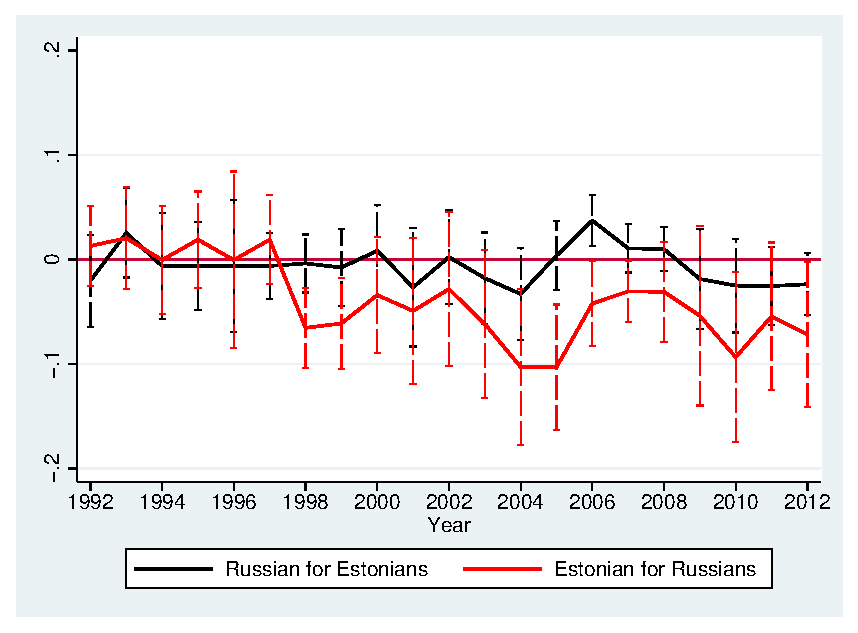
\includegraphics[width=0.45\linewidth]{Figure2a.eps}

		\label{fig:long-run_unemployment_estonian_russian_men}
	}
	\subfigure[Non-native languages for women]{      
		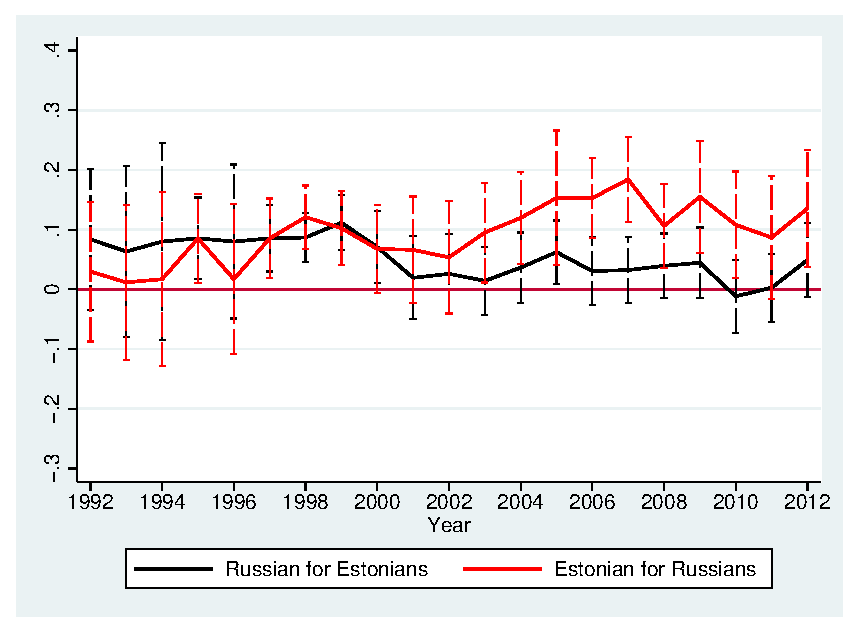
\includegraphics[width=0.45\linewidth]{Figure2b.eps}
		\label{fig:long-run_unemployment_estonian_russian_women}
	}
	\subfigure[English for Men]{
		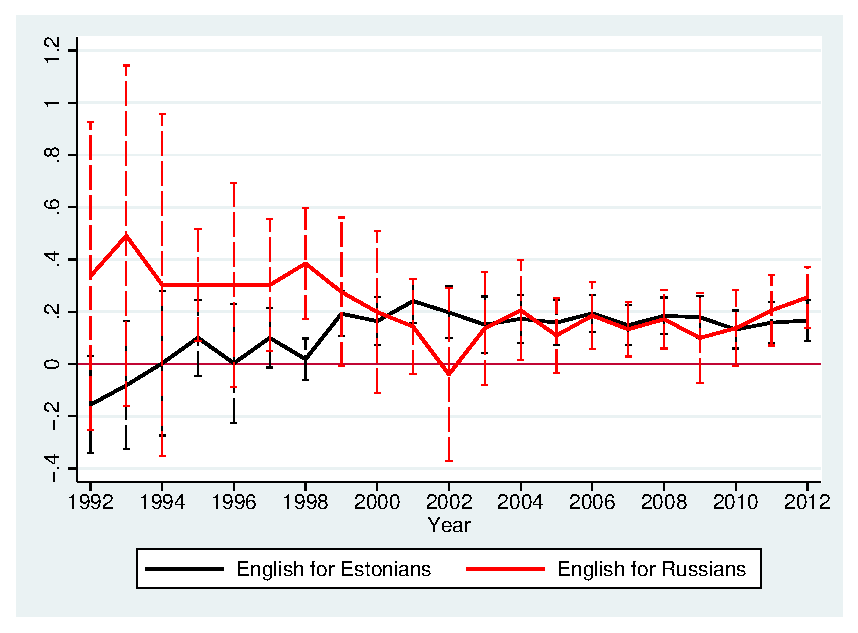
\includegraphics[width=0.45\linewidth]{Figure2c.eps}
		\label{fig:long-run_unemployment_english_men}
	}
	\subfigure[English for Women]{
		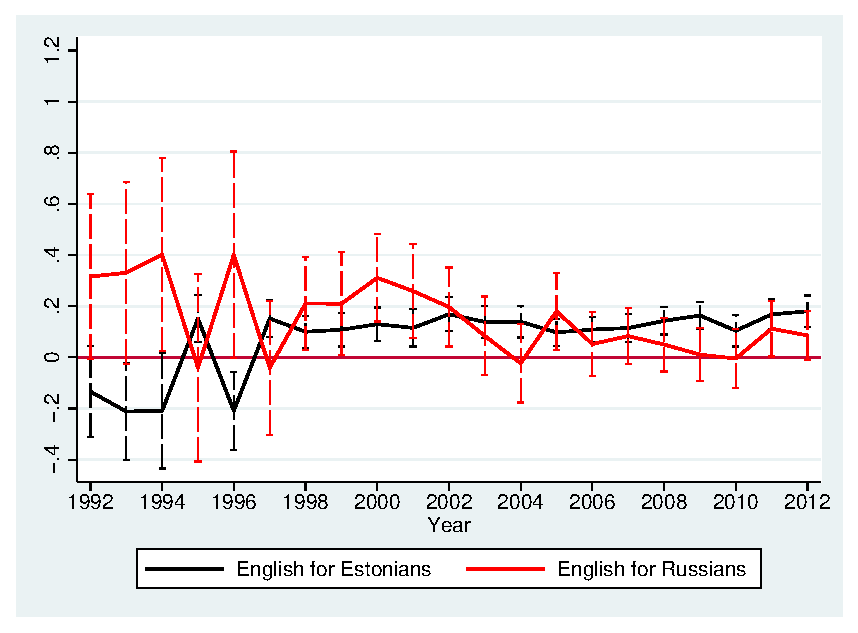
\includegraphics[width=0.45\linewidth]{Figure2d.eps}
		\label{fig:long-run_unemployment_english_women}
	}
	\caption{The effect of language fluency on unemployment, 1992--2012. \\ Control variables are \modelTwo. \agerestrictions }
	\label{fig:long-run_unemployment}
\end{figure}

For Estonian men, fluency in English is associated with less unemployment through the whole
period of observation whereas fluency in Russian has no effect.
Only a few of the results are pointwise statistically significant though.
For Estonian women, both languages are associated with less
unemployment in the 1990s but not later. The picture is different for
Russians. For men, we cannot see any substantial effect of fluency in English
whereas fluency in Estonian is clearly associated with less unemployment from
the late 1990s on. For women, the picture is mostly similar, just the
effect of Estonian language fluency seems to be somewhat delayed compared to
that for men.

\begin{figure}[htb]
	\centering
	\subfigure[Non-native languages for men]{
		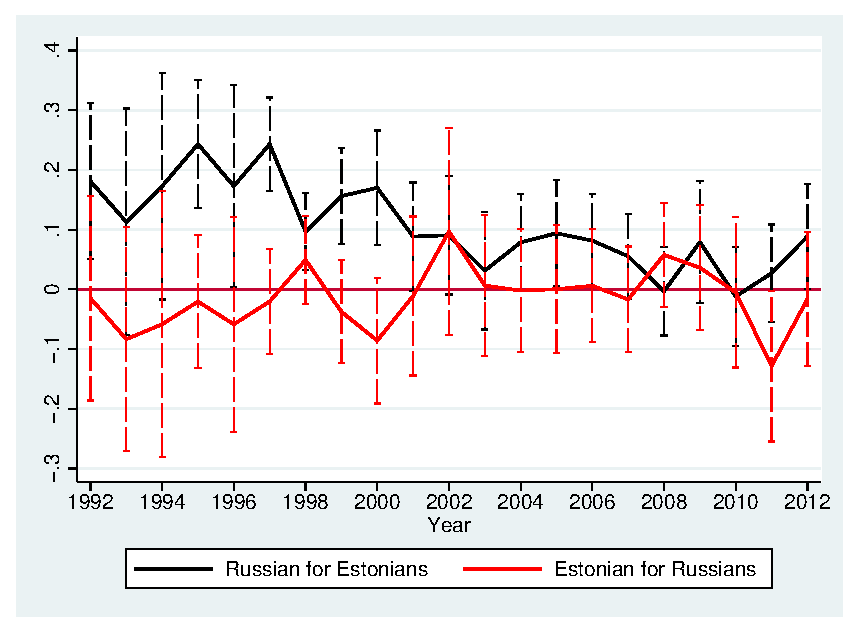
\includegraphics[width=0.45\linewidth]{Figure3a.eps}
		\label{fig:long-run_wage_estonian_russian_men}
	}
	\subfigure[Non-native languages for women]{
		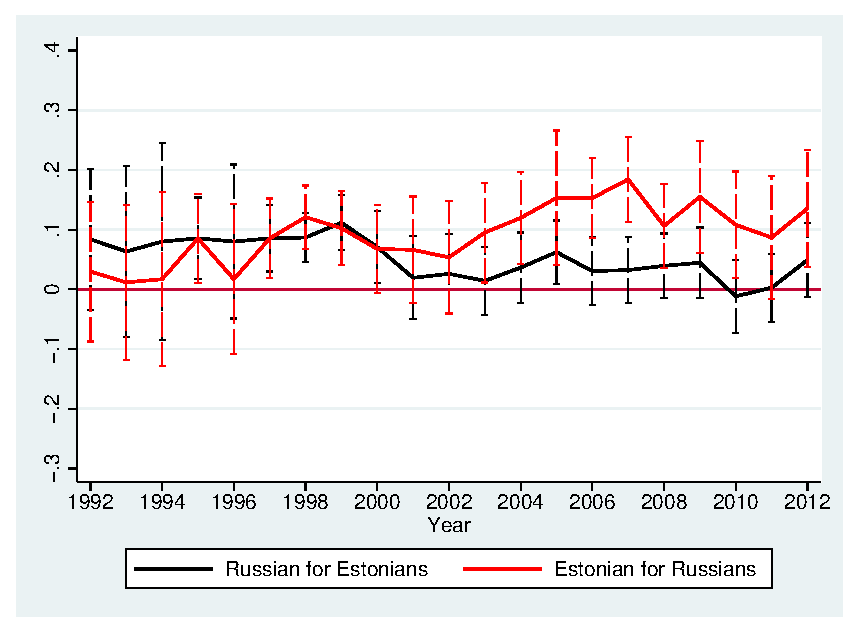
\includegraphics[width=0.45\linewidth]{Figure3b.eps}
		\label{fig:long-run_wage_estonian_russian_women}
	}
	\subfigure[English for Men]{
		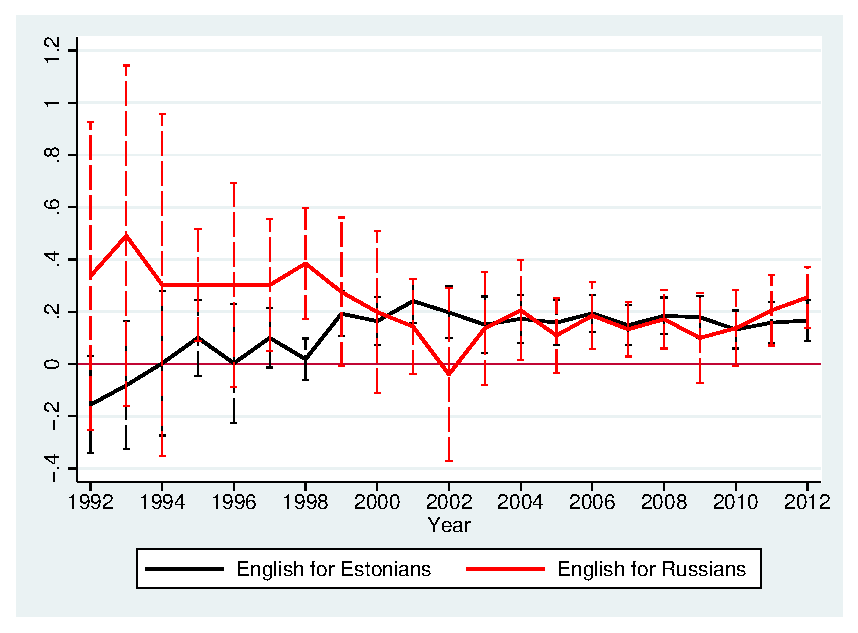
\includegraphics[width=0.45\linewidth]{Figure3c.eps}
		\label{fig:long-run_wage_english_men}
	}
	\subfigure[English for Women]{
		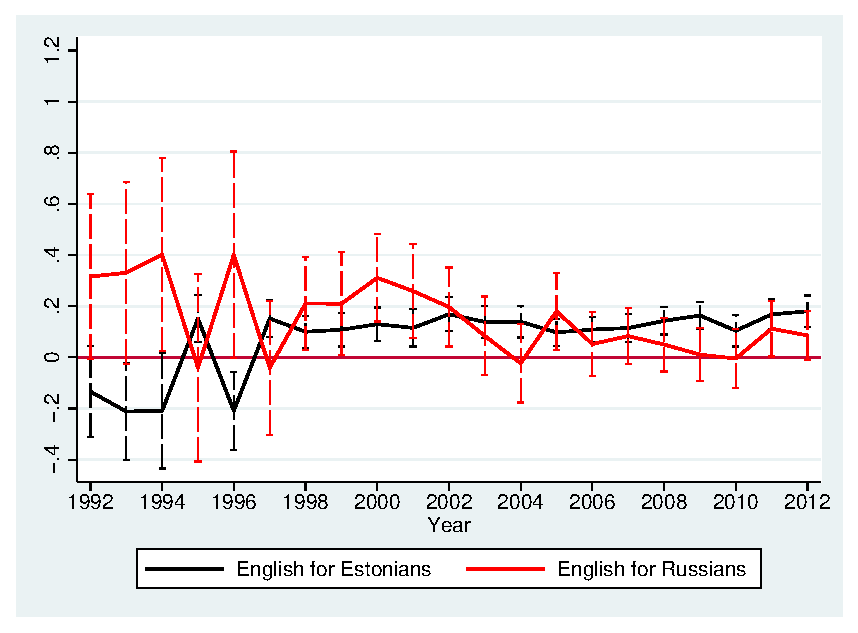
\includegraphics[width=0.45\linewidth]{Figure3d.eps}
		\label{fig:long-run_wage_english_women}
	}
	\caption{The effect of language fluency on wage, 1992--2012. \\ Control variables are \modelTwo. \agerestrictions}
	\label{fig:long-run_wage}
\end{figure}

The wage effects show a similar smooth long-term trend. For Estonians, we
see a slowly fading effect of Russian fluency whereas
English becomes important in the late 1990s. For Russian men, fluency in Estonian
has never been significantly associated with a wage premium.
The results are remarkably stable over the whole period, indicating
that the peculiar labour market institutions have been persistent for
two decades. However, for women we can see that Estonian language fluency turned
important in the late 1990s, suggesting that there is either less
workplace segregation or another kind of necessity to know the official
language at
the jobs commonly taken by women. The
importance of English seems to be falling over time for Russians, possibly
due to the increasing supply of these skills. 


\subsection{Does the Effect Differ by Age?}
\label{sec:age_groups}
As age is a central determinant of how major economic and political
reforms influence individual careers, 
we also analyse the time trends by age groups
(Table~\ref{tab:age_group_trend}).
We group the observation period into 4 sub-periods: early transition
(1989--1995); first economic growth (1996--1999);
the economic boom, EU accession (2000--2007); and the recession
(2008--2012).
We use the same econometric framework as described in section
\ref{sec:method}, the results presented here are based on the specification 2.

For ethnic Estonians, knowledge of Russian
(Table~\ref{tab:age_group_trend}, upper panel) has become less
important after its peak in the late 1990s. Notably, the
association between wage and language skills are small in the
young groups, the age groups where knowledge of that language
declining rapidly.
For older age groups, the estimates are larger but not statistically
significant since the recession period. English was not important
during the early years of transition but has been very closely
associated with better pay since 1996. Its importance seems to
fall for the young and middle male groups while the oldest men
(45-55) and the youngest women (25-35) show a growing trend.
This result potentially reflects both the changing supply and demand for 
English.

Now we turn to ethnic Russians (lower panel in the table). The association between Estonian skills and income shows no
statistically significant results at all. This is the most unexpected
outcome in our analysis, and we'll return to this
below in Section~\ref{sec:segregation-analysis}.
The effect of Estonian language skills was initially small for Russian
women as well, but
since the year 2000, we observe a sizeable gain of approximately
10\% for all subgroups.
The positive outcomes for women for the second decade in our analysis
suggests that the previously segregated ``Estonian'' and ``Russian''
economies are slowly becoming a more integrated one where ethnic
Russians, at least women, with good Estonian command get better-paid
jobs than those who cannot speak the language.
In comparison, the estimates for the English language skills trend downward over
time for all age groups for both men and for women. A likely
cause is the increasing abundance of these skills over time.

\begin{table}[htbp]
	\centering
	\caption{The trend over time across the age groups (ethnic Estonians)}
	\begin{tabular}{lccc|cc c}
     \toprule
		\multicolumn{7}{l}{Estonian speakers. Dependent variable: log wage}     \\ \hline
		Russian:  &  \multicolumn{3}{c|}{Men}  &  \multicolumn{3}{c}{Women}  \\
		years/age: & 25-35  & 36-45  & 46-55  & 25-35  & 36-45  & 46-55  \\ \midrule
		89-95   & 0.064  & 0.247*** & 0.187*** & 0.117*  & 0.033  & 0.058  \\
		      & (0.069) & (0.068) & (0.064) & (0.053) & (0.057) & (0.056) \\
		96-99   & 0.116** & 0.161** & 0.190*** & 0.059*  & 0.114*** & 0.131*** \\
		      & (0.042) & (0.049) & (0.054) & (0.030) & (0.030) & (0.033) \\
		00-07   & 0.054*  & 0.157*** & 0.093*  & 0.041  & 0.022  & 0.042  \\
		      & (0.026) & (0.037) & (0.037) & (0.024) & (0.021) & (0.026) \\
		08-12   & 0.041  & 0.032  & 0.088  & 0.032  & 0.012  & 0.061  \\
		      & (0.032) & (0.049) & (0.069) & (0.030) & (0.026) & (0.033) \\ \hline
		English:  &     &     &     &     &     &     \\
		89-95   & 0.097  & -0.008  & 0.066  & 0.070  & 0.042  & 0.101  \\
		      & (0.064) & (0.065) & (0.083) & (0.049) & (0.048) & (0.078) \\
		96-99   & 0.190*** & 0.276*** & 0.137*  & 0.113*** & 0.101*** & 0.101** \\
		      & (0.036) & (0.049) & (0.054) & (0.031) & (0.028) & (0.038) \\
		00-07   & 0.166*** & 0.158*** & 0.225*** & 0.159*** & 0.073*** & 0.164*** \\
		      & (0.027) & (0.036) & (0.041) & (0.024) & (0.021) & (0.025) \\
		08-12   & 0.088*  & 0.179*** & 0.236*** & 0.166*** & 0.123*** & 0.145*** \\
		      & (0.039) & (0.035) & (0.043) & (0.037) & (0.024) & (0.029) \\ 
     \midrule
		\multicolumn{7}{l}{Russian speakers. Dependent variable: log wage}\\
		\midrule
		Estonian:&\multicolumn{3}{c|}{Men} &\multicolumn{3}{c}{Women}\\
		years/age: & 25-35  & 36-45  & 46-55  & 25-35  & 36-45  & 46-55  \\
		\midrule
		89-95   & -0.027 & -0.113  & -0.029 & 0.134* & 0.073  & -0.039  \\
		      & (0.094) & (0.077) & (0.079) & (0.056) & (0.052) & (0.059) \\
		96-99   & -0.023 & 0.001  & 0.049  & 0.049  & 0.034  & 0.071  \\
		      & (0.050) & (0.048) & (0.060) & (0.045) & (0.035) & (0.037) \\
		00-07   & -0.038 & -0.034  & 0.042  & 0.099** & 0.089** & 0.122*** \\
		      & (0.038) & (0.049) & (0.043) & (0.033) & (0.031) & (0.028) \\
		08-12   & -0.004 & -0.034  & 0.002  & 0.145** & 0.123** & 0.103** \\
		      & (0.055) & (0.050) & (0.047) & (0.051) & (0.044) & (0.038) \\ \midrule
		English:  &     &     &     &     &     & 
           \\
     
		89-95   & 0.325* & 0.362*  & 0.473* & 0.191  & 0.096  & -0.096  \\
		      & (0.160) & (0.151) & (0.216) & (0.104) & (0.085) & (0.353) \\
		96-99   & 0.324** & 0.224*  & 0.129  & 0.241** & 0.048  & 0.281*  \\
		      & (0.101) & (0.103) & (0.132) & (0.078) & (0.091) & (0.120) \\
		00-07   & 0.142** & 0.107  & 0.169* & 0.127** & 0.104  & 0.127*  \\
		      & (0.051) & (0.097) & (0.072) & (0.049) & (0.060) & (0.057) \\
		08-12   & 0.140* & 0.212*** & 0.138  & 0.029  & 0.105* & 0.040  \\
		      & (0.056) & (0.057) & (0.072) & (0.049) & (0.050) & (0.055) \\
		\bottomrule
	\end{tabular}

	\caption*{\legend \\ Standard errors (clustered on individuals) in parentheses. \\ Individual characteristics are \modelTwo. 	}
	\label{tab:age_group_trend}
\end{table}

We repeat the exercise for the unemployment models.
However, due to relatively small groups, most of the results are not
statistically significant and we
do not report those here.



\section{Additional Evidence: Education and Workplace}
\label{sec:segregation-analysis}

The most surprising result in our analysis so far -- the fact that
Russian men earn virtually no Estonian language premium while women do -- warrants a
deeper look at the data. We split the average wage for the Russian male wage-earners
along three
dimensions: Estonian language skills (\emph{EST 0} and \emph{EST 1}),
residence in Tallinn metro area (\emph{Tallinn} and \emph{Other}),
and education (\emph{< HS}, \emph{HS}, \emph{College Degree}). The metropolitan area is one of the two major regions
where the Russian-speaking population is concentrated, and its
booming economy may be very different from the other such region, the
North-East (Ida-Virumaa), and the rest of the country.
In order to correct for the strong wage and language skill trends
through the observation period, we do not present the average wage,
but instead the respective OLS residuals where we explain the log wage by year fixed
effects and include no other explanatory variables (Table~\ref{tab:loc-lang-edu}). 

The table shows that the picture is in fact complex. We can see
that there is little to no gain from Estonian skills for the
largest group of workers, those with a high school degree. Even more, outside of
the metropolitan area, the lowest and highest education groups
have in fact negative language premium. However, these two groups
enjoy quite a noticeable premium in the Tallinn region. The
opposite-signed effects in for these two education groups suggests
that a
selective internal migration may play a role.

% latex table generated in R 3.4.4 by xtable 1.8-2 package
% Fri Jul 6 15:59:47 2018
\begin{table}[ht]
 \centering
 \caption{Average wage and time-trend corrected residual across
  location and education groups for Russian men}
 \begin{tabular}{llrrrr}
  \toprule
  & & &\multicolumn{2}{c}{Log Wage}\\
  Location & Education & \# Observations & EST 0 & EST 1 & Premium\\
  \midrule
  Tallinn & $<$ HS & 399 & -0.20 & -0.01 & 0.19 \\ 
  Tallinn & HS & 2,164 & 0.07 & 0.04 & -0.03 \\ 
  Tallinn & College Degree & 610 & 0.15 & 0.30 & 0.15 \\ 
  Other & $<$ HS & 501 & -0.12 & -0.12 & -0.01 \\ 
  Other & HS & 2,658 & -0.10 & -0.07 & 0.03 \\ 
  Other & College Degree & 429 & 0.17 & 0.11 & -0.06 \\ 
  \bottomrule
 \end{tabular}
 \begin{flushleft}
  Notes: \emph{Log Wage} refers to regression residual where log
  wage is explained by year fixed effects. \emph{EST 0} and
  \emph{EST 1} are mean values for those who cannot, and who can,
  speak Estonian; $\text{Premium} = \text{EST 1} - \text{EST 0}$.
  Education level \emph{< HS} refers to less than high school
  degree, \emph{HS} is the high school degree as the highest
  completed education.
 \end{flushleft}
 \label{tab:loc-lang-edu}
\end{table}

We can conclude from the Table~\ref{tab:loc-lang-edu} that our
most surprising finding, no positive effect of Estonian language
skills for Russian men, is primarily driven by the largest group, workers with
a high school degree. It also suggests that highly educated workers in
the metropolitan area enjoy, in fact, a substantial language premium.
However, this group is not very large.

The previous results can be explained by a combination of two hypotheses: first,
Russian--speaking men, at least those with high school degree as their
highest completed education level, are working
primarily in Russian language environment (ethnic segregation) while this is not true for
women; and second, Russian-speaking men are working in jobs with
little communication requirements (gender segregation).
To get some additional evidence on these hypotheses, we use data
from the 2008 Integration Monitor Survey. We focus on
two questions: ``which is the language of communication at your
workplace?'' and ``which languages do you need at work''. The first
question addresses the ethnic segregation while the second focuses on
the need of the language for communication. 

\begin{table}[t]         
	\centering
	\caption{Language environment and language need at workplace}
	\label{tab:environment_descriptive}
	\begin{tabular}{lrr}
		\toprule
		                   & men & women \\
		\midrule
		main communication language Estonian & 15.0 & 22.2 \\
		Need Estonian at work        & 53.0 & 61.9 \\
		Need English at work        & 26.5 & 11.9 \\
		\midrule
		\# Observations             & 132 & 134  \\
		\bottomrule
	\end{tabular}
	\begin{flushleft}
		Note: percentage of respondents who respond affirmatively
	\end{flushleft}
\end{table}

Table~\ref{tab:environment_descriptive} shows the proportion of
Russian respondents who use Estonian as the main communication language at work, and
who need Estonian and English at work. As we see, women are more likely to
use Estonian while the opposite is true for English.
Table~\ref{tab:environment_model} presents the corresponding regression results
where we estimate the likelihood of having the need for and using the
language at work
while
controlling for gender and other individual
characteristics, including education and geographic location.

\begin{table}[t]
	\centering
	\caption{Language environment and language need at workplace:
		regression results}
	\label{tab:environment_model}
	\begin{tabular}{l r@{}l r@{}l r@{}l}
		\toprule
		Dependent variable: & \multicolumn{2}{c}{Need Estonian} & \multicolumn{2}{c}{Use Estonian} & \multicolumn{2}{c}{Need English} \\ \midrule
		woman       & 0.262    & ** & 0.162    & *  & -0.045   &  \\
		         & \std{0.117} &   & \std{0.095} &   & \std{0.192} &  \\
		college education & 0.201    & ** & 0.132    & ** & 0.133    & * \\
		         & \std{0.083} &   & \std{0.067} &   & \std{0.079} &  \\
		region Tallinn  & -0.276   & *** & -0.463   & *** & 0.036    &  \\
		         & \std{0.083} &   & \std{0.067} &   & \std{0.080} &  \\
		region North-East & -0.527   & *** & -0.473   & *** & 0.022    &  \\
		         & \std{0.091} &   & \std{0.074} &   & \std{0.088} &  \\ \midrule
		\# Observations       & 228     &   & 228     &   & 228     &  \\
		$R^{2}$      & 0.2598   &   & 0.2831   &   & 0.108    &  \\ \bottomrule
	\end{tabular}
	\begin{flushleft}
		Note: control variables include: marital status, education,
		occupation and age.
	\end{flushleft}
\end{table}

The table indicates that Russian women need Estonian 26 percentage
points more at work than Russian men. The table also suggests that
Russian women are 16 percentage points more likely to be working in
Estonian-speaking environment when controlling for other factors.
Both figures are statistically significant (at 5\% and 10 \% level
respectively), although the standard errors are large. We can also see that
college education is associated with much more Estonian need and usage,
but in regions where large amounts of Russian speakers live, the capital
Tallinn and the North-East, Estonian is less needed. In contrast, no
gender difference is visible for English needs.

In summary, this dataset supports both of the hypotheses outlined above: Russian women are
working in a less segregated environment where Estonian is the main
communication language and they need Estonian at work for other reasons as
well. Gender differences in English usage are not statistically
significant.


\section{Discussion and Concluding Remarks}
\label{sec:discussion}

We document that all analysed language skills are associated with
unemployment and wage, however in different ways. Our most
intriguing observation is that the largest group of
Russian men, high school graduates, earn virtually no income premium if fluent in Estonian,
the majority and the official language of the country, while ability
to speak the language is related to a substantially
lower unemployment rate.
Our analysis supports \citet{YaoandOurs2015}, and \citet{Lindemann2013} findings that 
the labour market is segmented between ethnic and gender lines.
However, we find that ethnic segregation is less prevalent in the male
labour market.
This suggests for the majority of Russian-speaking men, Estonian
language gives a distinct advantage by facilitating hiring by
Estonian-dominated employers. We also confirm
\citet{leppik+vihalemm2015JofBaltStud} conclusion that
these
jobs are associated with little career mobility. There is also some
anecdotal evidence suggesting that offices are
typically manned by ethnic Estonians while manufacturing units have a
large share of Russian workers.
One can speculate that this outcome is related to a substantial population share
with negative attitudes toward Russians \citep{korts2009JofBaltStud}.
On a more positive tone, we find
that this may not be the case for highly educated workers.

The ethnic segregation seems to be less of an issue for women.
Unfortunately, neither \citet{Toomet2011} nor
\citet{leppik+vihalemm2015JofBaltStud} analyse men and women
separately. We find some evidence that female labour market is less
segregated along ethnic lines, and women are more frequently employed in jobs in which they need Estonian
language more, such as working in a direct contact with customers.
We also find evidence that over time Estonian is becoming more
important in the female labour market. Unfortunately, the current data
does not let us assess whether this is due to decreasing segregation, or
economy--wide rise of the importance of Estonian language. No such trend is visible for
men suggesting that 20 years ---almost a generation--- after
establishing a nation-state and market economy, the
labour market integration is still not complete.

The fact that the Russian language is not associated with any better
employment prospects
is in stark contrast to the results by \citet{Alan2015}. This is
potentially related to the sharp re-orientation to Western markets and
nation-state related political reforms Estonia experienced in the
early 1990s. Rapid withdrawal from the former USSR economy has
resulted in
a laudable economic growth, but may have led to
increased ethnic disparities, compared to the economies that moved in
a slower pace, such as Ukraine \citep{Constant2011} and the former Caucasus republics
\citep{Alan2015}. 

Our other results are more in line with other studies.
English language fluency is related to a substantial income premium but
to virtually no effect on unemployment. This is similar to findings by
\citet{ginsburgh+prieto-rodriguez2011ILRR} and \cite{fabo+2017E}
who show that English is more important at better-paid
jobs. In contrast, our outcomes suggest that English has little use
at unstable jobs, at these jobs where workers frequently move between
employment and unemployment.
Note also that in case of
English, we are able to explain a substantial part of the raw effect
by individual characteristics, suggesting that the true causal effect
may be smaller than our estimates.

The study has two main limitations. Although we believe that our
estimates are good indicators of a causal relationship, we cannot be
sure this is the case as our data do not contain strong enough instruments.
In particular, as individual characteristics are able to explain a
large part of English returns, we suppose part of the remaining effect
may also be related to an ability bias. Another weak point in the current
data are the self-reported language
skills. As language test data becomes available, we may be able to
decrease the measurement error in the future.


\bibliographystyle{apacite}
\bibliography{literatur}
\clearpage
\appendix
%appendix.tex
%Will contain potential additional tables and graphs
%\appendix
\FloatBarrier
\section{Additional tables}
\subsection{Different sample sizes}
%Copied from the original table, because it does not have the same number of Observations per model
\begin{table}[H]
	\begin{center}
		\caption{Estimation results for unemployment.}
		\label{tab:unemployment_estimation_by_sex_and_ethnic}
		\begin{tabular}{l D{.}{.}{3} @{\qquad} D{.}{.}{3} @{\qquad\qquad}
				D{.}{.}{3} @{\qquad} D{.}{.}{3}}
			\toprule
			&         \multicolumn{2}{c}{Men}         &        \multicolumn{2}{c}{Women}        \\
			Estonians:      & \multicolumn{1}{c}{1}      & \multicolumn{1}{l}{\hspace{10pt}2} & \multicolumn{1}{c}{1}      & \multicolumn{1}{c}{2}      \\
			Russian         & -0.026^{***}               & -0.010                             & -0.009^{*}                 & 0.010^{**}                 \\
			& (0.006)                    & (0.006)                            & (0.005)                    & (0.005)                    \\
			English         & -0.047^{***}               & -0.019^{***}                       & -0.024^{***}               & -0.008^{*}                 \\
			& (0.004)                    & (0.005)                            & (0.004)                    & (0.004)                    \\
			\# Observations          & \multicolumn{1}{c}{36,160} & \multicolumn{1}{l}{36,132}         & \multicolumn{1}{l}{36,050} & \multicolumn{1}{c}{36,015} \\
			$R^{2}$         & 0.022                      & 0.047                              & 0.012                      & 0.036                      \\ \hline
			Russians: & \\
			Estonian        & -0.052^{***}               & -0.052^{***}                       & -0.065^{***}               & -0.045^{***}               \\
			& (0.010)                    & (0.011)                            & (0.009)                    & (0.010)                    \\
			English         & -0.020                     & 0.006                              & -0.015                     & -0.003                     \\
			& (0.012)                    & (0.014)                            & (0.011)                    & (0.012)                    \\
			\# Observations          & \multicolumn{1}{c}{12,946} & \multicolumn{1}{l}{12,942}         & \multicolumn{1}{l}{13,689} & \multicolumn{1}{c}{13,674} \\
			$R^{2}$         & 0.033                      & 0.066                              & 0.023                      & 0.043                      \\ \hline
			year dummies    & \V                         & \V                                 & \V                         & \V                         \\
			indiv. charact. &                            & \V                                 &                            & \V                         \\
			\bottomrule
		\end{tabular}%
		\begin{flushleft}
			\caption*{ \legend \\ Standard errors (clustered on individuals) in parentheses.\\  Individual characteristics are \modelTwo. \\ \restrictions}
		\end{flushleft}
	\end{center}
	
\end{table}%

\begin{table}[htbp]
	\begin{center}
		\caption{Estimation results for log wage}
		\label{tab:wage_estimation_by_sex_and_ethnic} %SKB 04.07.2018 14:22:Not yet updated only prepared
		%Modified to account for occupation
		\begin{tabular}{l | D{.}{.}{3} @{\qquad} D{.}{.}{3} @{\qquad} D{.}{.}{3}  @{\qquad} | @{\qquad}
				D{.}{.}{3} @{\qquad} D{.}{.}{3} @{\qquad} D{.}{.}{3}}
			\toprule
			&                                   \multicolumn{3}{c}{Men}                                    &                              \multicolumn{3}{c}{Women}                               \\
			Estonians          & \multicolumn{1}{c}{1}      & \multicolumn{1}{c}{2}      & \multicolumn{1}{l}{\hspace{10pt}3} & \multicolumn{1}{c}{1}      & \multicolumn{1}{c}{2}      & \multicolumn{1}{c}{3}      \\\midrule
			Russian            & 0.107^{***}                & 0.072^{***}                & 0.045^{***}                        & 0.096^{***}                & 0.041^{***}                & 0.016^{***}                \\
			& (0.015)                    & (0.015)                    & (0.013)                            & (0.011)                    & (0.011)                    & (0.009)                    \\
			English            & 0.343^{***}                & 0.162^{***}                & 0.108^{***}                        & 0.311^{***}                & 0.131^{***}                & 0.075^{***}                \\
			& (0.013)                    & (0.015)                    & (0.013)                            & (0.010)                    & (0.010)                    & (0.009)                    \\
			\# Observations             & \multicolumn{1}{l}{22,290} & \multicolumn{1}{l}{22,274} & \multicolumn{1}{l}{21,785}         & \multicolumn{1}{l}{26,673} & \multicolumn{1}{l}{26,644} & \multicolumn{1}{c}{26,449} \\
			$R^{2}$            & 0.726                      & 0.755                      & 0.801                              & 0.769                      & 0.810                      & 0.850                      \\ \midrule
			Russians:          &  \\
			Estonian           & 0.018                      & -0.014                     & -0.009                              & 0.167^{***}                & 0.114^{***}                & 0.066^{***}                \\
			& (0.018)                    & (0.019)                    & (0.018)                            & (0.014)                    & (0.014)                    & (0.012)                    \\
			English            & 0.249^{***}                & 0.155^{***}                & 0.103^{***}                        & 0.223^{***}                & 0.089^{***}                & 0.054^{***}                \\
			& (0.026)                    & (0.027)                    & (0.025)                            & (0.021)                    & (0.022)                    & (0.020)                    \\
			\# Observations             & \multicolumn{1}{l}{8234}   & \multicolumn{1}{l}{8233}   & \multicolumn{1}{l}{7978}           & \multicolumn{1}{l}{9904}   & \multicolumn{1}{l}{9895}   & \multicolumn{1}{c}{9697}   \\
			$R^{2}$            & 0.731                      & 0.746                      & 0.795                              & 0.794                      & 0.809                      & 0.855                      \\ \hline
			year dummies       & \V                         & \V                         & \V                                 & \V                         & \V                         & \V                         \\
			indiv. charact.    &                            & \V                         & \V                                 &                            & \V                         & \V                         \\
			workplace charact. &                            &                            & \V                                 &                            &                            & \V                         \\ \bottomrule
		\end{tabular}
		\begin{flushleft}
			\caption*{\legend \\ Standard errors (clustered on individuals) in parenthesis \\ Individual characteristics are \modelTwo. \\ Workplace characteristics are \modelThreeAdd. \\ \restrictions}
		\end{flushleft}
	\end{center}
\end{table}
\clearpage

\subsection{All coefficients table}

\subsubsection{Dependent Variable: Unemployment}
\label{sec:unemployment_full}
\begin{sidewaystable}
	

\begin{tabular}{l*{2}{c}| *{2}{c}| *{2}{c}| *{2}{c}}
			\toprule
	& \multicolumn{2}{c|}{Estonian Men} & \multicolumn{2}{c|}{Estonian Women} & \multicolumn{2}{c|}{Russian Men} & \multicolumn{2}{c}{Russian Women} \\ 
%	\midrule

	
	&\multicolumn{1}{c}{Model 1}&\multicolumn{1}{c|}{Model 2}&\multicolumn{1}{c}{Model 1}&\multicolumn{1}{c|}{Model 2}&\multicolumn{1}{c}{Model 1}&\multicolumn{1}{c|}{Model 2}&\multicolumn{1}{c}{Model 1}&\multicolumn{1}{c}{Model 2}\\
	\midrule
	fluent in Russian   &      -0.026\sym{***}&      -0.010         &      -0.009         &       0.010\sym{*}  &                     &                     &                     &                     \\

	&     (0.006)         &     (0.006)         &     (0.005)         &     (0.005)         &                     &                     &                     &                     \\		fluent in Estonian  &                     &                     &                     &                     &      -0.052\sym{***}&      -0.052\sym{***}&      -0.065\sym{***}&      -0.045\sym{***}\\
		&                     &                     &                     &                     &     (0.010)         &     (0.011)         &     (0.009)         &     (0.010)         \\
	fluent in English   &      -0.047\sym{***}&      -0.019\sym{***}&      -0.024\sym{***}&      -0.008         &      -0.020         &       0.006         &      -0.015         &      -0.003         \\
	&     (0.004)         &     (0.005)         &     (0.004)         &     (0.004)         &     (0.012)         &     (0.014)         &     (0.011)         &     (0.012)         \\
	age                 &                     &       0.001         &                     &      -0.017\sym{***}&                     &       0.004         &                     &      -0.004         \\
	&                     &     (0.003)         &                     &     (0.003)         &                     &     (0.006)         &                     &     (0.006)         \\
	age\sym{2}    &                     &       0.000         &                     &       0.000\sym{***}&                     &      -0.000         &                     &       0.000         \\
	&                     &     (0.000)         &                     &     (0.000)         &                     &     (0.000)         &                     &     (0.000)         \\
			Education &&&&&\\
	<=basic             &                     &       0.061\sym{***}&                     &       0.068\sym{***}&                     &       0.053\sym{***}&                     &       0.097\sym{***}\\
	&                     &     (0.007)         &                     &     (0.009)         &                     &     (0.015)         &                     &     (0.020)         \\
	college             &                     &      -0.028\sym{***}&                     &      -0.036\sym{***}&                     &      -0.053\sym{***}&                     &      -0.032\sym{**} \\
	&                     &     (0.005)         &                     &     (0.004)         &                     &     (0.012)         &                     &     (0.011)         \\
	Married             &                     &      -0.054\sym{***}&                     &      -0.023\sym{***}&                     &      -0.118\sym{***}&                     &      -0.045\sym{***}\\
	&                     &     (0.005)         &                     &     (0.004)         &                     &     (0.012)         &                     &     (0.009)         \\
	Number of Children  &                     &      -0.008\sym{***}&                     &       0.014\sym{***}&                     &      -0.002         &                     &       0.018\sym{**} \\
	&                     &     (0.002)         &                     &     (0.002)         &                     &     (0.006)         &                     &     (0.007)         \\
	Harju county \& Tallinn&                     &       0.045\sym{***}&                     &       0.060\sym{***}&                     &       0.118\sym{**} &                     &       0.094\sym{*}  \\
	&                     &     (0.013)         &                     &     (0.013)         &                     &     (0.039)         &                     &     (0.048)         \\
	Ida-Viru county   &                     &       0.084\sym{***}&                     &       0.091\sym{***}&                     &       0.131\sym{***}&                     &       0.129\sym{**} \\
	&                     &     (0.020)         &                     &     (0.020)         &                     &     (0.039)         &                     &     (0.048)         \\
	Rest of Estonia   &                     &       0.065\sym{***}&                     &       0.081\sym{***}&                     &       0.143\sym{***}&                     &       0.079         \\
	&                     &     (0.013)         &                     &     (0.013)         &                     &     (0.041)         &                     &     (0.048)         \\
	Interethnic Household&                     &       0.039\sym{***}&                     &       0.020         &                     &      -0.014         &                     &       0.001         \\
	&                     &     (0.012)         &                     &     (0.011)         &                     &     (0.015)         &                     &     (0.013)         \\


	Constant            &       0.163\sym{***}&       0.072         &       0.106\sym{***}&       0.357\sym{***}&       0.203\sym{***}&       0.067         &       0.225\sym{***}&       0.221         \\
	&     (0.009)         &     (0.057)         &     (0.007)         &     (0.054)         &     (0.013)         &     (0.118)         &     (0.014)         &     (0.126)         \\
	year dummies        &         Yes         &         Yes         &         Yes         &         Yes         &         Yes         &         Yes         &         Yes         &         Yes         \\
	\midrule
\#	Observations        &       36160         &       36132         &       36050         &       36015         &       12946         &       12942         &       13689         &       13674         \\
	Adjusted \(R^{2}\)  &       0.022         &       0.047         &       0.012         &       0.035         &       0.032         &       0.065         &       0.022         &       0.041         \\
	\bottomrule
	\multicolumn{9}{l}{\footnotesize Standard errors in parentheses}\\
	\multicolumn{9}{l}{\footnotesize \sym{*} \(p<0.05\), \sym{**} \(p<0.01\), \sym{***} \(p<0.001\)}
\end{tabular}
\end{sidewaystable}
\clearpage

\subsubsection{Dependent Variable: Log Wage}
\label{sec:wage_full}


	\begin{longtable}{l*{3}{c}|l*{3}{c}}
%		\caption{Estimation results for log wage: all coefficients}
		\toprule
		& \multicolumn{3}{c|}{Estonian Men} & \multicolumn{3}{c}{Estonian Women} \\
				&\multicolumn{1}{c}{Model 1}&\multicolumn{1}{c}{Model 2}&\multicolumn{1}{c|}{Model 3}&\multicolumn{1}{c}{Model 1}&\multicolumn{1}{c}{Model 2}&\multicolumn{1}{c}{Model 3}\\ 
				\midrule
		\endfirsthead
		\toprule
				& \multicolumn{3}{c|}{Estonian Men} & \multicolumn{3}{c}{Estonian Women} \\
		&\multicolumn{1}{c}{Model 1}&\multicolumn{1}{c}{Model 2}&\multicolumn{1}{c|}{Model 3}&\multicolumn{1}{c}{Model 1}&\multicolumn{1}{c}{Model 2}&\multicolumn{1}{c}{Model 3}\\
		\midrule
		\endhead
		\midrule
		\endfoot
		\bottomrule
		\endlastfoot
%		&\multicolumn{1}{c}{Model 1}&\multicolumn{1}{c}{Model 2}&\multicolumn{1}{c}{Model 3}&\multicolumn{1}{c}{Model 1}&\multicolumn{1}{c}{Model 2}&\multicolumn{1}{c}{Model 3}\\
%		\midrule
		fluent in Russian   &       0.107\sym{***}&       0.072\sym{***}&       0.044\sym{**} &       0.096\sym{***}&       0.041\sym{***}&       0.016         \\
		&     (0.015)         &     (0.015)         &     (0.013)         &     (0.011)         &     (0.011)         &     (0.009)         \\
		fluent in English   &       0.343\sym{***}&       0.162\sym{***}&       0.108\sym{***}&       0.311\sym{***}&       0.131\sym{***}&       0.075\sym{***}\\
		&     (0.013)         &     (0.015)         &     (0.013)         &     (0.010)         &     (0.010)         &     (0.009)         \\
		age                 &                     &       0.023\sym{**} &       0.020\sym{**} &                     &       0.045\sym{***}&       0.030\sym{***}\\
		&                     &     (0.007)         &     (0.006)         &                     &     (0.006)         &     (0.005)         \\
		age\textsuperscript{2}    &                     &      -0.000\sym{***}&      -0.000\sym{***}&                     &      -0.001\sym{***}&      -0.000\sym{***}\\
		&                     &     (0.000)         &     (0.000)         &                     &     (0.000)         &     (0.000)         \\
		Education &&&&&\\
		<=basic             &                     &      -0.147\sym{***}&      -0.084\sym{***}&                     &      -0.163\sym{***}&      -0.083\sym{***}\\
		&                     &     (0.014)         &     (0.013)         &                     &     (0.014)         &     (0.013)         \\
		college             &                     &       0.269\sym{***}&       0.215\sym{***}&                     &       0.360\sym{***}&       0.228\sym{***}\\
		&                     &     (0.017)         &     (0.017)         &                     &     (0.011)         &     (0.011)         \\
		married           &                     &       0.127\sym{***}&       0.082\sym{***}&                     &      -0.005         &      -0.012         \\
		&                     &     (0.012)         &     (0.011)         &                     &     (0.009)         &     (0.008)         \\
		Number of Children         &                     &       0.021\sym{***}&       0.015\sym{**} &                     &      -0.035\sym{***}&      -0.023\sym{***}\\
		&                     &     (0.005)         &     (0.005)         &                     &     (0.005)         &     (0.004)         \\
		Harju county  \& Tallinn      &                     &      -0.649\sym{***}&      -0.547\sym{***}&                     &      -0.967\sym{***}&      -1.093\sym{***}\\
		&                     &     (0.078)         &     (0.100)         &                     &     (0.105)         &     (0.130)         \\
		IdaViru           &                     &      -0.852\sym{***}&      -0.691\sym{***}&                     &      -1.265\sym{***}&      -1.298\sym{***}\\
		&                     &     (0.084)         &     (0.104)         &                     &     (0.109)         &     (0.132)         \\
		Rest of Estonia&                     &      -0.858\sym{***}&      -0.680\sym{***}&                     &      -1.216\sym{***}&      -1.263\sym{***}\\
		&                     &     (0.078)         &     (0.100)         &                     &     (0.105)         &     (0.130)         \\
		Interethnic Household        &                     &      -0.047\sym{*}  &      -0.054\sym{*}  &                     &      -0.064\sym{**} &      -0.047\sym{*}  \\
		&                     &     (0.023)         &     (0.021)         &                     &     (0.023)         &     (0.020)         \\
		Industry &&&&&\\
		B                   &                     &                     &       0.146\sym{*}  &                     &                     &       0.001         \\
		&                     &                     &     (0.074)         &                     &                     &     (0.113)         \\
		C                   &                     &                     &       0.050         &                     &                     &      -0.008         \\
		&                     &                     &     (0.029)         &                     &                     &     (0.034)         \\
		D                   &                     &                     &       0.075\sym{***}&                     &                     &       0.046         \\
		&                     &                     &     (0.020)         &                     &                     &     (0.029)         \\
		E                   &                     &                     &       0.141\sym{***}&                     &                     &       0.157\sym{**} \\
		&                     &                     &     (0.036)         &                     &                     &     (0.048)         \\
		F                   &                     &                     &       0.278\sym{***}&                     &                     &       0.053         \\
		&                     &                     &     (0.022)         &                     &                     &     (0.043)         \\
		G                   &                     &                     &       0.145\sym{***}&                     &                     &       0.025         \\
		&                     &                     &     (0.024)         &                     &                     &     (0.028)         \\
		H                   &                     &                     &       0.153\sym{***}&                     &                     &       0.048         \\
		&                     &                     &     (0.035)         &                     &                     &     (0.033)         \\
		I                   &                     &                     &       0.265\sym{***}&                     &                     &       0.033         \\
		&                     &                     &     (0.024)         &                     &                     &     (0.033)         \\
		J                   &                     &                     &       0.190\sym{**} &                     &                     &       0.083         \\
		&                     &                     &     (0.063)         &                     &                     &     (0.043)         \\
		K                   &                     &                     &       0.075\sym{*}  &                     &                     &       0.049         \\
		&                     &                     &     (0.032)         &                     &                     &     (0.034)         \\
		L                   &                     &                     &       0.150\sym{***}&                     &                     &       0.124\sym{***}\\
		&                     &                     &     (0.033)         &                     &                     &     (0.034)         \\
		M                   &                     &                     &      -0.020         &                     &                     &      -0.053         \\
		&                     &                     &     (0.040)         &                     &                     &     (0.032)         \\
		N                   &                     &                     &      -0.034         &                     &                     &      -0.003         \\
		&                     &                     &     (0.049)         &                     &                     &     (0.031)         \\
		O                   &                     &                     &       0.050         &                     &                     &      -0.036         \\
		&                     &                     &     (0.033)         &                     &                     &     (0.033)         \\
		P                   &                     &                     &      -0.139\sym{*}  &                     &                     &      -0.126\sym{**} \\
		&                     &                     &     (0.071)         &                     &                     &     (0.038)         \\
		Q                   &                     &                     &       0.014         &                     &                     &       0.005         \\
		&                     &                     &     (0.103)         &                     &                     &     (0.047)         \\
		R                   &                     &                     &      -0.057         &                     &                     &      -0.103\sym{*}  \\
		&                     &                     &     (0.102)         &                     &                     &     (0.044)         \\
		S                   &                     &                     &      -0.087         &                     &                     &      -0.039         \\
		&                     &                     &     (0.111)         &                     &                     &     (0.088)         \\
				U                   &                     &                     &                     &                     &                     &       0.049         \\
		&                     &                     &                     &                     &                     &     (0.145)         \\
		Occupation &&&&&\\
		1                   &                     &                     &       0.187\sym{***}&                     &                     &       0.211\sym{**} \\
		&                     &                     &     (0.032)         &                     &                     &     (0.067)         \\
		2                   &                     &                     &       0.034         &                     &                     &       0.119         \\
		&                     &                     &     (0.034)         &                     &                     &     (0.066)         \\
		3                   &                     &                     &      -0.019         &                     &                     &      -0.009         \\
		&                     &                     &     (0.032)         &                     &                     &     (0.066)         \\
		4                   &                     &                     &      -0.146\sym{***}&                     &                     &      -0.160\sym{*}  \\
		&                     &                     &     (0.039)         &                     &                     &     (0.067)         \\
		5                   &                     &                     &      -0.251\sym{***}&                     &                     &      -0.228\sym{***}\\
		&                     &                     &     (0.034)         &                     &                     &     (0.067)         \\
		6                   &                     &                     &      -0.084         &                     &                     &      -0.084         \\
		&                     &                     &     (0.049)         &                     &                     &     (0.074)         \\
		7                   &                     &                     &      -0.072\sym{*}  &                     &                     &      -0.151\sym{*}  \\
		&                     &                     &     (0.033)         &                     &                     &     (0.069)         \\
		8                   &                     &                     &      -0.099\sym{**} &                     &                     &      -0.225\sym{***}\\
		&                     &                     &     (0.032)         &                     &                     &     (0.067)         \\
		9                   &                     &                     &      -0.374\sym{***}&                     &                     &      -0.378\sym{***}\\
		&                     &                     &     (0.036)         &                     &                     &     (0.067)         \\
		Ownership form &&&&&\\
		20                  &                     &                     &      -0.161\sym{***}&                     &                     &      -0.078\sym{***}\\
		&                     &                     &     (0.026)         &                     &                     &     (0.014)         \\
		30                  &                     &                     &      -0.068\sym{**} &                     &                     &       0.021         \\
		&                     &                     &     (0.026)         &                     &                     &     (0.023)         \\
		40                  &                     &                     &       0.224\sym{***}&                     &                     &       0.185\sym{***}\\
		&                     &                     &     (0.028)         &                     &                     &     (0.026)         \\
		50                  &                     &                     &       0.369\sym{**} &                     &                     &       0.133         \\
		&                     &                     &     (0.140)         &                     &                     &     (0.078)         \\
		90                  &                     &                     &       0.881\sym{*}  &                     &                     &       0.385\sym{***}\\
		&                     &                     &     (0.406)         &                     &                     &     (0.084)         \\
		nWorkers            &                     &                     &       0.043\sym{***}&                     &                     &       0.046\sym{***}\\
		&                     &                     &     (0.003)         &                     &                     &     (0.002)         \\
		publicSector      &                     &                     &      -0.038         &                     &                     &      -0.006         \\
		&                     &                     &     (0.029)         &                     &                     &     (0.022)         \\
		experienceInCompany &                     &                     &       0.002         &                     &                     &       0.011\sym{***}\\
		&                     &                     &     (0.002)         &                     &                     &     (0.002)         \\
		experienceInCompany\textsuperscript{2}&                     &                     &      -0.000         &                     &                     &      -0.000\sym{***}\\
		&                     &                     &     (0.000)         &                     &                     &     (0.000)         \\
		Constant            &       7.863\sym{***}&       8.351\sym{***}&       8.122\sym{***}&       7.610\sym{***}&       8.009\sym{***}&       8.266\sym{***}\\
		&     (0.021)         &     (0.153)         &     (0.160)         &     (0.016)         &     (0.154)         &     (0.183)         \\
		year dummies        &         Yes         &         Yes         &         Yes         &         Yes         &         Yes         &         Yes         \\
		\midrule
	\#	Observations        &       22290         &       22274         &       21785         &       26673         &       26644         &       26449         \\
		Adjusted \(R^{2}\)  &       0.726         &       0.755         &       0.801         &       0.769         &       0.810         &       0.850         \\
		\bottomrule
		\multicolumn{7}{l}{\footnotesize Standard errors in parentheses}\\
		\multicolumn{7}{l}{\footnotesize \sym{*} \(p<0.05\), \sym{**} \(p<0.01\), \sym{***} \(p<0.001\)}
          \label{tab:et_wage_full}
	\end{longtable}

\clearpage

	\begin{longtable}{l*{3}{c}|l*{3}{c}}
		\toprule
				& \multicolumn{3}{c|}{Russian Men} & \multicolumn{3}{c}{Russian Women} \\
				&\multicolumn{1}{c}{Model 1}&\multicolumn{1}{c}{Model 2}&\multicolumn{1}{c|}{Model 3}&\multicolumn{1}{c}{Model 1}&\multicolumn{1}{c}{Model 2}&\multicolumn{1}{c}{Model 3}\\
						\midrule
		\endfirsthead
		\toprule
						& \multicolumn{3}{c|}{Russian Men} & \multicolumn{3}{c}{Russian Women} \\
				&\multicolumn{1}{c}{Model 1}&\multicolumn{1}{c}{Model 2}&\multicolumn{1}{c|}{Model 3}&\multicolumn{1}{c}{Model 1}&\multicolumn{1}{c}{Model 2}&\multicolumn{1}{c}{Model 3}\\
						\midrule
		\endhead
		\midrule
		\endfoot
		\bottomrule
		\endlastfoot


		fluent in Estonian  &       0.018         &      -0.014         &      -0.009         &       0.167\sym{***}&       0.114\sym{***}&       0.066\sym{***}\\
		&     (0.018)         &     (0.019)         &     (0.018)         &     (0.014)         &     (0.014)         &     (0.013)         \\
		fluent in English   &       0.249\sym{***}&       0.155\sym{***}&       0.103\sym{***}&       0.223\sym{***}&       0.089\sym{***}&       0.054\sym{**} \\
		&     (0.026)         &     (0.027)         &     (0.025)         &     (0.021)         &     (0.022)         &     (0.018)         \\
		age                 &                     &       0.024\sym{*}  &       0.012         &                     &       0.014         &       0.008         \\
		&                     &     (0.010)         &     (0.009)         &                     &     (0.008)         &     (0.007)         \\
		age\textsuperscript{2}   &                     &      -0.000\sym{**} &      -0.000         &                     &      -0.000\sym{*}  &      -0.000         \\
		&                     &     (0.000)         &     (0.000)         &                     &     (0.000)         &     (0.000)         \\
		Education &&&&&\\
		<=basic             &                     &      -0.084\sym{***}&      -0.051\sym{*}  &                     &      -0.034         &       0.017         \\
		&                     &     (0.024)         &     (0.022)         &                     &     (0.023)         &     (0.020)         \\
		college             &                     &       0.181\sym{***}&       0.100\sym{***}&                     &       0.272\sym{***}&       0.125\sym{***}\\
		&                     &     (0.027)         &     (0.026)         &                     &     (0.019)         &     (0.018)         \\
		Married           &                     &       0.139\sym{***}&       0.102\sym{***}&                     &      -0.021         &      -0.032\sym{**} \\
		&                     &     (0.021)         &     (0.018)         &                     &     (0.013)         &     (0.011)         \\
		Number of Children         &                     &       0.009         &       0.011         &                     &      -0.007         &      -0.003         \\
		&                     &     (0.011)         &     (0.009)         &                     &     (0.009)         &     (0.008)         \\
		Harju county \& Tallinn&                     &      -0.722\sym{***}&      -0.603\sym{**} &                     &      -1.222\sym{***}&      -1.298\sym{***}\\
		&                     &     (0.184)         &     (0.216)         &                     &     (0.159)         &     (0.117)         \\
		Ida-Viru county   &                     &      -0.824\sym{***}&      -0.778\sym{***}&                     &      -1.338\sym{***}&      -1.463\sym{***}\\
		&                     &     (0.184)         &     (0.215)         &                     &     (0.159)         &     (0.118)         \\
		Rest of Estonia   &                     &      -0.813\sym{***}&      -0.690\sym{**} &                     &      -1.290\sym{***}&      -1.372\sym{***}\\
		&                     &     (0.185)         &     (0.216)         &                     &     (0.159)         &     (0.118)         \\
		Interethnic Household&                     &       0.062\sym{*}  &       0.067\sym{*}  &                     &       0.019         &       0.020         \\
		&                     &     (0.031)         &     (0.026)         &                     &     (0.023)         &     (0.019)         \\
		Industry &&&&&\\
		B                   &                     &                     &       0.328\sym{**} &                     &                     &       0.162         \\
		&                     &                     &     (0.104)         &                     &                     &     (0.099)         \\
		C                   &                     &                     &       0.221\sym{**} &                     &                     &      -0.013         \\
		&                     &                     &     (0.071)         &                     &                     &     (0.066)         \\
		D                   &                     &                     &       0.098         &                     &                     &      -0.031         \\
		&                     &                     &     (0.067)         &                     &                     &     (0.060)         \\
		E                   &                     &                     &       0.118         &                     &                     &       0.033         \\
		&                     &                     &     (0.072)         &                     &                     &     (0.071)         \\
		F                   &                     &                     &       0.277\sym{***}&                     &                     &       0.065         \\
		&                     &                     &     (0.069)         &                     &                     &     (0.083)         \\
		G                   &                     &                     &       0.067         &                     &                     &      -0.037         \\
		&                     &                     &     (0.071)         &                     &                     &     (0.062)         \\
		H                   &                     &                     &       0.259\sym{**} &                     &                     &      -0.042         \\
		&                     &                     &     (0.082)         &                     &                     &     (0.064)         \\
		I                   &                     &                     &       0.240\sym{***}&                     &                     &       0.037         \\
		&                     &                     &     (0.070)         &                     &                     &     (0.064)         \\
		J                   &                     &                     &       0.447\sym{**} &                     &                     &       0.181         \\
		&                     &                     &     (0.145)         &                     &                     &     (0.093)         \\
		K                   &                     &                     &       0.045         &                     &                     &      -0.142\sym{*}  \\
		&                     &                     &     (0.074)         &                     &                     &     (0.068)         \\
		L                   &                     &                     &       0.099         &                     &                     &       0.018         \\
		&                     &                     &     (0.088)         &                     &                     &     (0.080)         \\
		M                   &                     &                     &      -0.049         &                     &                     &      -0.120         \\
		&                     &                     &     (0.094)         &                     &                     &     (0.066)         \\
		N                   &                     &                     &      -0.069         &                     &                     &      -0.070         \\
		&                     &                     &     (0.098)         &                     &                     &     (0.065)         \\
		O                   &                     &                     &      -0.024         &                     &                     &      -0.076         \\
		&                     &                     &     (0.087)         &                     &                     &     (0.066)         \\
		P                   &                     &                     &      -0.353         &                     &                     &      -0.185\sym{*}  \\
		&                     &                     &     (0.330)         &                     &                     &     (0.089)         \\
		Q                   &                     &                     &      -0.045         &                     &                     &       0.019         \\
		&                     &                     &     (0.192)         &                     &                     &     (0.075)         \\
		R                   &                     &                     &       0.054         &                     &                     &      -0.240         \\
		&                     &                     &     (0.263)         &                     &                     &     (0.195)         \\
		S                   &                     &                     &       0.095         &                     &                     &       0.044         \\
		&                     &                     &     (0.189)         &                     &                     &     (0.123)         \\
		Occupation &&&&&\\
		1                   &                     &                     &      -0.005         &                     &                     &       0.089         \\
		&                     &                     &     (0.075)         &                     &                     &     (0.062)         \\
		2                   &                     &                     &      -0.137         &                     &                     &       0.074         \\
		&                     &                     &     (0.074)         &                     &                     &     (0.058)         \\
		3                   &                     &                     &      -0.215\sym{**} &                     &                     &      -0.099         \\
		&                     &                     &     (0.071)         &                     &                     &     (0.053)         \\
		4                   &                     &                     &      -0.296\sym{***}&                     &                     &      -0.208\sym{***}\\
		&                     &                     &     (0.081)         &                     &                     &     (0.056)         \\
		5                   &                     &                     &      -0.462\sym{***}&                     &                     &      -0.310\sym{***}\\
		&                     &                     &     (0.067)         &                     &                     &     (0.059)         \\
		6                   &                     &                     &      -0.403\sym{**} &                     &                     &      -0.138         \\
		&                     &                     &     (0.127)         &                     &                     &     (0.094)         \\
		7                   &                     &                     &      -0.307\sym{***}&                     &                     &      -0.197\sym{***}\\
		&                     &                     &     (0.069)         &                     &                     &     (0.057)         \\
		8                   &                     &                     &      -0.298\sym{***}&                     &                     &      -0.238\sym{***}\\
		&                     &                     &     (0.069)         &                     &                     &     (0.055)         \\
		9                   &                     &                     &      -0.548\sym{***}&                     &                     &      -0.440\sym{***}\\
		&                     &                     &     (0.071)         &                     &                     &     (0.054)         \\
		Ownership form &&&&&\\

		20                  &                     &                     &      -0.179\sym{***}&                     &                     &      -0.028         \\
		&                     &                     &     (0.038)         &                     &                     &     (0.026)         \\
		30                  &                     &                     &      -0.117\sym{***}&                     &                     &      -0.041         \\
		&                     &                     &     (0.026)         &                     &                     &     (0.027)         \\
		40                  &                     &                     &       0.020         &                     &                     &       0.064\sym{*}  \\
		&                     &                     &     (0.030)         &                     &                     &     (0.030)         \\
		50                  &                     &                     &      -0.069         &                     &                     &       0.213\sym{*}  \\
		&                     &                     &     (0.139)         &                     &                     &     (0.095)         \\
		90                  &                     &                     &      -0.001         &                     &                     &      -0.138         \\
		&                     &                     &     (0.191)         &                     &                     &     (0.471)         \\
		nWorkers            &                     &                     &       0.032\sym{***}&                     &                     &       0.030\sym{***}\\
		&                     &                     &     (0.004)         &                     &                     &     (0.003)         \\
		publicSector      &                     &                     &      -0.021         &                     &                     &       0.011         \\
		&                     &                     &     (0.041)         &                     &                     &     (0.032)         \\
		experienceInCompany &                     &                     &       0.011\sym{***}&                     &                     &       0.013\sym{***}\\
		&                     &                     &     (0.003)         &                     &                     &     (0.002)         \\
		experienceInCompany\textsuperscript{2}&                     &                     &      -0.000\sym{*}  &                     &                     &      -0.000\sym{***}\\
		&                     &                     &     (0.000)         &                     &                     &     (0.000)         \\
		Constant            &       7.918\sym{***}&       8.208\sym{***}&       8.430\sym{***}&       7.535\sym{***}&       8.570\sym{***}&       8.925\sym{***}\\
		&     (0.023)         &     (0.268)         &     (0.300)         &     (0.018)         &     (0.218)         &     (0.202)         \\
		year dummies        &         Yes         &         Yes         &         Yes         &         Yes         &         Yes         &         Yes         \\
		\midrule
	\#	Observations        &        8234         &        8233         &        7977         &        9904         &        9895         &        9697         \\
		Adjusted \(R^{2}\)  &       0.731         &       0.745         &       0.793         &       0.793         &       0.809         &       0.854         \\
		\bottomrule
		\multicolumn{7}{l}{\footnotesize Standard errors in parentheses}\\
		\multicolumn{7}{l}{\footnotesize \sym{*} \(p<0.05\),
          \sym{**} \(p<0.01\), \sym{***} \(p<0.001\)}
          \label{tab:ru_wage_full}
	\end{longtable}



\end{document}
